\chapter{Model błędu wyniku pomiaru}

Aby określić w jakim stopniu analizowany tor pomiarowy spełnia powierzone mu zadanie pomiarowe należy ilościowo przedstawić przedział, w którym z określonym prawdopodobieństwem będą znajdowały się wartości wielkości wyjściowych tego toru pomiarowego~\cite{jcgm_guide}. Należy zatem zdefiniować w jaki sposób rozumiana jest idealna wartość wielkości wyjściowej, a następnie zdefiniować różnicę pomiędzy rzeczywistą i idealną wartością wielkości wyjściowej nazywaną w dalszej części pracy błędem wielkości wyjściowej. Zakładając, że proces uzyskiwania wartości wielkości wyjściowej będzie powtarzany wielokrotnie, opisaną różnicę można analizować probabilistycznie, przedstawiając jej parametry za pomocą funkcji gęstości prawdopodobieństwa. W przypadku, gdy analizowany tor pomiarowy dostarcza na wyjściu wiele wielkości wyjściowych, każdą z nich należy analizować osobno. Istnieją jednak przypadki, w których analiza może odbywać się zbiorczo dla pewnej grupy wielkości wyjściowych, wykazującej identyczne właściwości metrologiczne~\cite{auth_electronics}.

Analizując tor pomiarowy przedstawiony na rysunku~\ref{fig:chain_demo}, z punktu widzenia pojedynczej wielkości wyjściowej, zauważyć można, że proces wyznaczania wielkości wyjściowej obejmuje trzy główne etapy: przetwarzanie analogowe, konwersje analogowo-cyfrową oraz przetwarzanie cyfrowe. Ze względu na możliwą zależność właściwości kolejnych części toru pomiarowego od widma przetwarzanego sygnału, analizę omawianych procesów należy rozpatrywać w dziedzinie częstotliwości~\cite{jakubiec_system}. Właściwości zależne od częstotliwości przetwarzanego sygnału mogą być zatem opisane w przypadku cześć analogowej za pomocą transmitancji $G_{y}(j\omega)$ oraz transmitancji $H_{X}(z)$ w przypadku części cyfrowej. Każda z omawianych części, poza odpowiednio wyrażoną transmitancją, charakteryzuje się związaną z nią funkcją przetwarzania, oznaczoną w przypadku części analogowej symbolem $f_{y}(x)$ oraz symbolem $f_{X}(x)$ w przypadku cześć cyfrowej. Funkcje te opisują, w jaki sposób element wyznacza wartość wielkości wyjściowej na podstawie wartości wielkości wejściowej. Pomiędzy częściami analogową i cyfrową znajduje się przetwornik analogowo-cyfrowy, przetwarzający sygnał $y(t)$ na jego dyskretną reprezentację $x(i)$. Schemat ideowy dla omawianego modelu toru pomiarowego przedstawiono na rysunku~\ref{fig:chain_trans}.

\begin{figure}[htb!]
\begin{center}
\includegraphics{obrazki/schemat_trans}
\makecaption{fig:chain_trans}{Schemat blokowy toru pomiarowego z punktu widzenia pojedynczej wielkości wyjściowej}
\end{center}
\end{figure}

Przedstawiony na rysunku~\ref{fig:chain_trans} przypadek zakłada, że przetwarzanie analogowo-cyfrowe przebiega w sposób idealny, tj. nie wprowadza do przetwarzanego sygnału żadnych błędów. Założenie to będzie oczywiście nieprawidłowe w rzeczywistym torze pomiarowym, dlatego sam przetwornik analogowo-cyfrowy również należy opisać za pomocą przedstawionego na rysunku~\ref{fig:chain_trans} modelu o parametrach odpowiednich dla analizowanego przetwornika. Naturalnie, tor pomiarowy składać się może z wielu elementów połączonych ze sobą szeregowo, które odpowiednio przetwarzać będą sygnał ciągły w czasie lub przetwarzać będą jego dyskretną reprezentacje. Należy zatem przedstawiać rzeczywisty tor pomiarowy jako połączenie kolejnych elementów o odpowiednich dla nich parametrach lub za pomocą modelu opisującego wypadkowe parametry wszystkich analizowanych części tego toru. W przypadku, gdy dla analizowanego fragmentu toru pomiarowego jego właściwości nie są istotne z punktu analizy metrologicznej, właściwości te można pominąć~\cite{jcgm_guide}.

Analizując właściwości metrologiczne elementów toru pomiarowego należy dokonać podziału ich cech ze względu na rolę w przetwarzaniu przez nie sygnału wejściowego. Część cech będzie bowiem użyteczna z punktu widzenia roli toru pomiarowego (np. wzmocnienie sygnału, filtracja sygnału), przy czym te same cechy mogą okazać się problematyczne i wprowadzać będą one do wielkości wyjściowej niepożądane z punktu widzenia realizowanego zadania błędy (np. filtracja sygnału, gdy nie jest pożądana, będzie ten sygnał tłumić i przesuwać w fazie). Każdy z fragmentów toru pomiarowego, zgodnie ze swoimi właściwościami, wprowadzać będzie do sygnału wyjściowego błędy własne oraz przenosić będzie na wyjście obecne w sygnale wejściowym błędy. Jak wcześniej wspomniano, nie wszystkie właściwości analizowanego elementu toru pomiarowego będą odpowiedzialne za wprowadzanie do wielkości wyjściowych błędów -- jeśli ich działanie jest pożądane, to przyjmuje się że realizują powierzone im zadanie przetwarzania sygnału. Dla przykładu, jeśli elementem toru pomiarowego jest wzmacniacz, to jego zadaniem jest wprowadzenie stałego wzmocnienia wielkości wejściowych niezależnie od widma sygnału wejściowego. Jeśli zatem element ten wprowadzi inne wzmocnienie, niż oczekiwane, lub też wpłynie on na widmo przetwarzanego sygnału, działanie to zostanie rozpatrzone jako niepożądane, a jego skutki zostaną opisane jako wprowadzenie błędu własnego do wielkości wyjściowej. Z drugiej strony, jeśli analizowanym elementem byłby filtr, to wprowadzenie tłumienia byłoby działaniem pożądanym i nie zostałoby opisane jako wprowadzenie błędu własnego do przetwarzanego sygnału -- chyba, że wprowadzone tłumienie posiadałoby parametry inne, niż oczekiwane. Należy zatem analizować właściwości kolejnych fragmentów toru pomiarowego w taki sposób, aby ocenić ich działanie pod kątem powierzonego im zadania przetworzenia wielkości wejściowych, a następnie określić, które ich cechy są pożądane, a które nie.

Ze względu na charakter, właściwości każdego z fragmentów toru pomiarowego podzielić można na dwie najważniejsze grupy:
\begin{description}
\item [Właściwości statyczne] w przypadku, gdy właściwości te nie są związane z widmem przetwarzanego sygnału wejściowego.
\item [Właściwości dynamiczne] w przypadku gdy właściwości te są bezpośrednio związane z widmem przetwarzanego sygnału.
\end{description}

Jako, że wybrane właściwości kolejnych fragmentów toru pomiarowego będą zależały od widma przetwarzanego sygnału, w dalszej cześć rozdziału przyjmuje się założenie, że niezakłócony błędami przetwarzany sygnał wejściowy $s(t)$ opisać można w postaci sumy kolejnych harmonicznych tego sygnału równaniem:
\begin{equation}
\dot{s} \emb{t} = \sum _{i = 0} ^{\infty} \dot{s} \left( t, \omega_{s,i} \right) \label{eq:in_cont_sum},
\end{equation}
przy czym $\omega_{s,i}$ jest pulsacją $i$-tej harmonicznej opisywanego sygnału oraz:
\begin{gather}
\dot{s} \left( t, \omega \right) = E_{s,o} \emb{\omega} \sin \left( \omega t + \varphi_{s,o} \emb{\omega} \right) \label{eq:in_cont_omega_ideal}, \\
\tilde{s} \left( t, \omega \right) = \dot{s} \left( t, \omega \right) + E_{s,e} \emb{\omega} \sin \left( \omega t + \varphi_{s,e} \emb{\omega} \right) \label{eq:in_cont_omega_real}, \\
\tilde{s} \emb{t} = e_{s,r} \emb{t} + \sum _{i = 0} ^{\infty} \tilde{s} \left( t, \omega_{s,i} \right) \label{eq:in_cont_sum_real},
\end{gather}
gdzie $E_{s,o}(\omega)$ jest amplitudą oraz $\varphi_{s,o}(\omega)$ przesunięciem w fazie wybranej harmonicznej sygnału w przypadku idealnym, $E_{s,e}(\omega)$ amplitudą oraz $ \varphi_{s,e}(\omega)$ przesunięciem w fazie analizowanej harmonicznej sygnału błędu, natomiast sygnał $e_{s,r}(t)$ jest błędem losowym. W równaniu~\eqref{eq:in_cont_sum_real} pominięto jawny opis składowej stałej sygnału, jako że zastąpić go można harmoniczną o indeksie $i = 0$, gdzie $\omega_{s,0} = 0$ oraz $\varphi_{s,0} = \pi$.

Na podstawie równania~\eqref{eq:in_cont_sum_real} wyróżnić można trzy grupy błędów, przy czym zaproponowany podział wynika z charakteru ich realizacji i obejmuje:
\begin{description}
\item [Błędy statyczne] dla których kolejne realizacje w obrębie pojedynczego okna pomiarowego nie zmieniają się lub zmieniają się nieznacznie.
\item [Błędy dynamiczne] dla których kolejne realizacje można opisać w sposób deterministyczny, jako sumę kolejnych harmonicznych tego błędu.
\item [Błędy losowe] dla których kolejne realizacje będą wynikały z reguł probabilistycznych, a zatem ich opis deterministyczny nie będzie możliwy.
\end{description}

Analizując przedstawione powyżej założenia oraz biorąc pod uwagę równania od~\eqref{eq:in_cont_sum} do~\eqref{eq:in_cont_sum_real}, wyróżnione błędy deterministyczne opisać można za pomocą równań:
\begin{gather}
e_{s,s} \emb{t} = E_{s,e} \emb{\omega_{s,0}} \sin \left( \omega_{s,0} t + \varphi_{s,e} \emb{\omega_{s,0}} \right) = E_{s,e} \emb{0} \label{eq:in_cont_err_stat}, \\
e_{s,d} \emb{t} = \sum _{i = 1} ^{\infty} E_{s,e} \emb{\omega_{s,i}} \sin \left( \omega_{s,i} t + \varphi_{s,e} \emb{\omega_{s,i}} \right) \label{eq:in_cont_err_dyn},
\end{gather}
gdzie symbolem $e_{s,s}(t)$ oznaczono błąd statyczny, natomiast symbolem $e_{s,d}(t)$ błąd dynamiczny zawarty w sygnale $s(t)$. Błąd wypadkowy $e_{s,\Sigma}(t)$ zawarty w sygnale $s(t)$ można zatem wyrazić w postaci sumy wszystkich wymienionych sygnałów błędów:
\begin{equation}
e_{s,\Sigma} \emb{t} = e_{s,s} \emb{t} + e_{s,d} \emb{t} + e_{s,r} \emb{t} \label{eq:in_cont_err_sum}.
\end{equation}

\section{Błędy w części analogowej toru pomiarowego}

Zgodnie z poprzednimi założeniami, aby ujednolicić analizę pojedynczego fragmentu części analogowej toru pomiarowego, element ten można przedstawić za pomocą transmitancji odpowiadającej właściwościom dynamicznym oraz odpowiedniej dla niego funkcji przetwarzania. Na rysunku~\ref{fig:chain_cont} przedstawiono schemat fragmentu części analogowej toru pomiarowego, którego cały schemat został przedstawiony na rysunku~\ref{fig:chain_trans}. W dalszej części podrozdziału zakłada się, że analizowany fragment toru pomiarowego przetwarza ciągły w czasie sygnał $s(t)$, opisany we wstępie rozdziału równaniami od~\eqref{eq:in_cont_sum} do~\eqref{eq:in_cont_sum_real}, na sygnał wyjściowy $y(t)$. Dodatkowo przyjmuje się, że funkcja $f_{y}(x)$ stanowi równanie przetwarzania opisywanego obiektu, natomiast transmitancja obiektu jest oznaczona symbolem $G_{u}(j\omega)$, przy czym jej wzmocnienie statyczne jest równe jedności oraz jej charakter jest liniowy i nie zależny w żaden sposób od czasu -- jest to zatem obiekt typu \enquote{LTI} (ang. \enquote{Linear time-invariant})~\cite{oppenheim_sns}.

\begin{figure}[htb!]
\begin{center}
\includegraphics{obrazki/schemat_ciagly}
\makecaption{fig:chain_cont}{Schemat blokowy pojedynczego fragmentu części analogowej toru pomiarowego}
\end{center}
\end{figure}

Błędy obecne w sygnale wyjściowym $y(t)$ podzielić można, podobnie jak we wprowadzeniu do rozdziału, na statyczne, dynamiczne i losowe. Podział ten natomiast należy rozszerzyć pod kątem genezy błędu, przy czym wyróżnione zostaną w tym przypadku błędy własne oraz propagowane. Jako błędy własne rozumie się te, które analizowany obiekt wprowadza do sygnału wyjściowego. Błędy propagowane są natomiast błędami zawartymi w sygnale wejściowym, przetworzonymi przez obiekt zgodnie z jego charakterystyką, a następnie przeniesionymi na wyjście tego obiektu. Suma sygnałów błędów własnych i propagowanych dla danej grupy błędów stanowi wypadkowy sygnał błędu tej grupy.

Pierwszy etap rozważań stanowi wpływ transmitancji $G_{u}(j\omega)$ analizowanego obiektu na błędy zawarte w wielkości wejściowej oraz jej rola we wprowadzaniu błędów własnych. W przypadku błędów statycznych, zgodnie z wprowadzonymi założeniami, transmitancja ta nie ma żadnego wpływu na obecne w sygnale wejściowym błędy statyczne oraz nie wprowadza własnego błędu statycznego. Przedstawione założenia mogą być opisane następującymi równaniami:
\begin{gather}
e_{u,sw} \emb{t} = 0 \label{eq:mid_cont_err_stat_self}, \\
e_{u,sp} \emb{t} = E_{s,s} \emb{0} \label{eq:mid_cont_err_stat_prop},
\end{gather}
gdzie $e_{u,sw}(t)$ jest błędem własnym, natomiast $e_{u,sp}(t)$ błędem przenoszonym przez fragment obiektu związany z jego właściwościami dynamicznymi.

Na podstawie transmitancji widmowej $G_{u}(j\omega)$ obiektu wyznaczyć można wzmocnienie $K_{u}(\omega)$ tego obiektu w funkcji pulsacji równe:
\begin{equation}
K_{u} \emb{\omega} = \left| G_{u} \emb{j\omega} \right| =
	\sqrt{\left( \Re \left( G_{u} \emb{j\omega} \right) \right)^{2} +
	\left( \Im \left( G_{u} \emb{j\omega} \right) \right)^{2}}
\label{eq:mid_cont_amp},
\end{equation}
oraz przesunięcie w fazie $\varphi_{u}(\omega)$ dla wybranej harmonicznej sygnału wejściowego dane zależnością:
\begin{equation}
\varphi_{u} \emb{\omega} = \arctan \left( \frac{\Im \left( G_{u} \emb{j\omega} \right)}{\Re \left( G_{u} \emb{j\omega} \right)} \right) \label{eq:mid_cont_phi}.
\end{equation}
Znajomość tych parametrów jest niezbędna do opisu sygnałów błędów dynamicznych własnych oraz propagowanych części związanej z transmitancją obiektu. Można jednak zauważyć, że bezpośrednia znajomość transmitancji widmowej obiektu nie jest konieczna, jeśli znane są przebiegi przedstawionych parametrów w funkcji częstotliwości.

Wprowadzanie przez analizowany obiekt błędów dynamicznych wynika z faktu, że rzeczywista transmitancja $\tilde{G}_{u}(j\omega)$ odbiega od transmitancji idealnej $\dot{G}_{u}(j\omega)$. Powoduje to, że obiekt ten wprowadza inne tłumienie i przesunięcie w fazie do kolejnych harmonicznych sygnału, niż wymagane dla realizowanego przez niego zadania pomiarowego. Rozpatrując pojedynczą harmoniczną sygnału $u(t)$, można opisać idealny przebieg tej harmonicznej w postaci równania:
\begin{equation}
\dot{u} \emb{t,\omega} = \dot{K}_{u} \emb{\omega} E_{s,o} \emb{\omega} \sin \left( \omega t + \varphi_{s,o} \emb{\omega} + \dot{\varphi}_{u} \emb{\omega} \right) \label{eq:mid_cont_omega_ideal},
\end{equation}
natomiast ten sam przebieg zakłócony błędami własnym i propagowanymi, wynikającymi z transmitancji obiektu, wyrazić można w postaci równania:
\begin{equation}
\begin{split}
\tilde{u} \emb{t,\omega} =~
& \tilde{K}_{u} \emb{\omega} E_{s,o} \emb{\omega} \sin \left( \omega t + \varphi_{s,o} \emb{\omega} + \tilde{\varphi}_{u} \emb{\omega} \right) + \\
& \tilde{K}_{u} \emb{\omega} E_{s,e} \emb{\omega} \sin \left( \omega t + \varphi_{s,e} \emb{\omega} + \tilde{\varphi}_{u} \emb{\omega} \right)
\end{split}
\label{eq:mid_cont_omega_real},
\end{equation}
Wobec powyższych zależności, wprowadzany do sygnału $u(t)$ błąd dynamiczny własny $e_{u,dw}(t)$ opisać można równaniem:
\begin{equation}
\begin{split}
e_{u,dw} \emb{t} =~
& \sum _{i = 1} ^{\infty} \tilde{K}_{u} \emb{\omega_{s,i}} E_{s,o} \emb{\omega_{s,i}} \sin \left( \omega_{s,i} t + \varphi_{s,o} \emb{\omega_{s,i}} + \tilde{\varphi}_{u} \emb{\omega_{s,i}} \right) - \\
& \sum _{i = 1} ^{\infty} \dot{K}_{u} \emb{\omega_{s,i}} E_{s,o} \emb{\omega_{s,i}} \sin \left( \omega_{s,i} t + \varphi_{s,o} \emb{\omega_{s,i}} + \dot{\varphi}_{u} \emb{\omega_{s,i}} \right)
\end{split}
\label{eq:mid_cont_err_dyn_self}.
\end{equation}
Poza wprowadzaniem do sygnału $u(t)$ błędu dynamicznego własnego, analizowany fragment obiektu przenosi z wejścia na wyjście błędy zawarte w sygnale wejściowym odpowiednio tłumiąc je i przesuwając w fazie:
\begin{equation}
e_{u,dp} \emb{t} = \sum _{i = 1} ^{\infty} \tilde{K}_{u} \emb{\omega_{s,i}} E_{s,e} \emb{\omega_{s,i}} \sin \left( \omega_{s,i} t + \varphi_{s,e} \emb{\omega_{s,i}} + \tilde{\varphi}_{u} \emb{\omega_{s,i}} \right) \label{eq:mid_cont_err_dyn_prop},
\end{equation}
przy czym $e_{u,dp}(t)$ jest sygnałem błędu dynamicznego, propagowanego z wejścia na wyjście fragmentu reprezentującego właściwości dynamiczne analizowanego obiektu.

Ostatnią grupę błędów dla analizowanego fragmentu obiektu stanowią błędy losowe. Błędów tych nie sposób opisać równaniem deterministycznym, a zatem opis ich właściwości sprowadza się do wskazania prawdopodobieństwa uzyskania wybranych wartości kolejnych realizacji tych błędów~\cite{jcgm_guide, jakubiec_system}. W dalszej cześć podrozdziału przyjmuje się założenie, że $\sigma_{s,r}^{2}(\omega)$ jest wariancją oraz $\sigma_{s,r}(\omega)$ odchyleniem standardowym błędu losowego zawartego w przetwarzanym sygnale wejściowym w funkcji pulsacji, oraz że kolejne wartości realizacji tego błędu nie są ze sobą skorelowane. Wobec powyższych założeń zauważyć można, że wpływ transmitancji $G_{u}(j\omega)$ na wejściowy sygnał błędu losowego zaowocuje pojawieniem się korelacji pomiędzy kolejnymi realizacjami sygnału błędu wyjściowego~\cite{jadziak_dsp, bibbona_filter, benassi_filter}. Zważywszy, że w praktyce każdy element toru pomiarowego posiada transmitancję różną od $G(j\omega) = \text{const}$, na jego wyjściu zwykle nie otrzymuje się sygnału błędu losowego o identycznej widmowej gęstości mocy, jak na wejściu. Wartość wariancji na wyjściu analizowanego fragmentu obiektu dla sygnału propagowanego błędu losowego w funkcji pulsacji opisać można równaniem~\cite{oppenheim_sns}:
\begin{equation}
\sigma_{u,rp}^{2} \emb{\omega} = \tilde{K}_{u}^{2} \emb{\omega} \sigma_{s,r}^{2} \emb{\omega} \label{eq:mid_cont_var_omega},
\end{equation}
natomiast średnią wartość wariancji $\overline{\sigma}_{u,rp}^{2}$ tego sygnału na wyjściu obiektu opisać można równaniem~\cite{jadziak_dsp, proakis_dsp}:
\begin{equation}
\overline{\sigma}_{u,rp}^{2} = \frac{1}{a - b} \int _{b} ^{a} \tilde{K}_{u}^{2} \emb{\omega} \sigma_{s,r}^{2} \emb{\omega} d\omega \label{eq:mid_cont_var_rand},
\end{equation}
przy czym $<a;b>$ jest zakresem częstotliwości, dla którego szacowana jest wariancja przenoszonego błędu losowego. W przypadku wystąpienia błędów losowych własnych również należy wskazać ich wariancję, opisaną jako $\sigma_{u,rw}^{2}(\omega)$. W przypadku kaskadowego połączenia kolejnych transmitancji należy wykorzystać właściwości transformacji Fouriera opisane w między innymi w podręcznikach~\cite{proakis_dsp, oppenheim_sns, oppenheim_dsp}.

Ostatecznie, sumując wszystkie sygnały błędów wielkości wyjściowej analizowanej części właściwości dynamicznych obiektu, otrzymuje się zależność opisującą wypadkowy sygnał błędu $e_{u,\Sigma}(t)$ w postaci równania:
\begin{equation}
e_{u,\Sigma} \emb{t} = e_{u,sp} \emb{t} + e_{u,dw} \emb{t} + e_{u,rw} \emb{t} + e_{u,dp} \emb{t} + e_{u,rp} \emb{t} \label{eq:mid_cont_err_sum_all}.
\end{equation}
Uwzględniając równanie przetwarzania $f_{y}(x)$ analizowanego obiektu zapisać można równanie przedstawiające idealną wielkość wyjściową obiektu jako:
\begin{equation}
\dot{y} \emb{t} = \dot{f}_{y} \left( \dot{s} \emb{t} \right) \label{eq:out_cont_ideal_all},
\end{equation}
natomiast, przy uwzględnieniu równania~\eqref{eq:mid_cont_err_sum_all}, wielkość tą obarczoną omówionymi błędami zapisać można w postaci:
\begin{equation}
\tilde{y} \emb{t} = \tilde{f}_{y} \left( \dot{s} \emb{t} + e_{u,\Sigma} \emb{t} \right) = \dot{y} \emb{t} + e_{y,\Sigma} \emb{t} \label{eq:out_cont_real_all}.
\end{equation}
Wypadkowy błąd wielkości wyjściowej analizowanego obiektu jest zatem dany równaniem:
\begin{equation}
e_{y,\Sigma} \emb{t} = \tilde{f}_{y} \left( \dot{s} \emb{t} + e_{u,\Sigma} \emb{t} \right) - \dot{f}_{y} \left( \dot{s} \emb{t} \right) + f_{z} \left( z_{1}, \hdots, z_{N} \right) \label{eq:out_cont_err_sum_all},
\end{equation}
przy czym $\tilde{f}_{y}(x)$ jest rzeczywistym, a $\dot{f}_{y}(x)$ idealnym równaniem przetwarzania obiektu, natomiast $f_{z}(\mathbf{z})$ jest funkcją uwzględniającą wybrane wielkości zakłócające.

Przypadek ogólny, przedstawiony w równaniach od~\eqref{eq:out_cont_ideal_all} do~\eqref{eq:out_cont_err_sum_all}, jest w praktyce trudny do rozważania. Nie gwarantuje on bowiem możliwości analizy każdego sygnału błędu cząstkowego z osobna i nie jest szczegółowo przedstawiony w niniejszej pracy. Dla przypadków, w których funkcja przetwarzania $f_{y}(x)$ jest addytywna, tj. spełnia założenie $f_{y}(a + b) = f_{y}(a) + f_{y}(b)$, gdzie $a$ oraz $b$ należą do dziedziny tej funkcji, opisywaną analizę można przeprowadzić z osobna dla każdego rodzaju błędów. Przedstawione założenie jest w praktyce często spełniane, ponieważ funkcja przetwarzania reprezentuje zwykle czułość obiektu w przypadku obiektów o charakterze liniowym, a zatem jest ona funkcją liniową wyrażoną w postaci równania $f(x) = ax$, gdzie współczynnik $a$ jest czułością obiektu. W dalszej części podrozdziału przyjęto założenie dotyczące addytywności funkcji $f_{y}(x)$, a następnie przedstawiono zależności wynikające z tego założenia.

W przypadku, gdy funkcja przetwarzania nie jest idealna, lub gdy istnieją pewne wielkości zakłócające, niebrane pod uwagę podczas pomiaru (np. wpływ ciśnienia, temperatury itp.), wyróżnić można dodatkowy wprowadzany błąd własny $e_{y,*w}(t)$, który opisać można równaniem:
\begin{equation}
e_{y,*w} \emb{t} = \tilde{f}_{y} \left( \dot{s} \emb{t} \right) - \dot{f}_{y} \left( \dot{s} \emb{t} \right) + f_{z} \left( z_{1}, \hdots, z_{N} \right) \label{eq:out_cont_err_stat_self},
\end{equation}
gdzie $\tilde{f}_{y}(x)$ jest rzeczywistą oraz $\dot{f}_{y}(x)$ idealną funkcją przetwarzania analizowanego obiektu, natomiast $f_{z}(\mathbf{z})$ jest funkcją opisującą wpływ wielkości zakłócających $\mathbf{z}$ na proces pomiaru. Należy zauważyć, że w skład sygnału błędu $e_{y,*w}(t)$ wchodzić mogą różne sygnały błędów, w tym o różnym charakterze. Pozostałe sygnały błędów wielkości $y(t)$, przy założeniu addytywności funkcji przetwarzania, opisać można za pomocą równań:
\begin{gather}
e_{y,sp} \emb{t} = \tilde{f}_{y} \left( e_{u,sp} \emb{t} \right) \label{eq:out_cont_err_stat_prop}, \\
e_{y,dw} \emb{t} = \tilde{f}_{y} \left( e_{u,dw} \emb{t} \right) \label{eq:out_cont_err_dyn_prop}, \\
e_{y,dp} \emb{t} = \tilde{f}_{y} \left( e_{u,dp} \emb{t} \right) \label{eq:out_cont_err_dyn_self}, \\
e_{y,rw} \emb{t} = \tilde{f}_{y} \left( e_{u,rw} \emb{t} \right) \label{eq:out_cont_err_rand_self}, \\
e_{y,rp} \emb{t} = \tilde{f}_{y} \left( e_{u,rp} \emb{t} \right) \label{eq:out_cont_err_rand_prop},
\end{gather}
przy czym kolejno $e_{y,sp}$ jest błędem statycznym propagowanym, $e_{y,dw}$ błędem dynamicznym własnym, $e_{y,dp}$ błędem dynamicznym propagowanym oraz $e_{y,rp}$ błędem losowym propagowanym wielkości wyjściowej obiektu. Wobec powyższych równań i przyjętych założeń, równanie~\eqref{eq:out_cont_err_sum_all} przyjmuje postać:
\begin{equation}
e_{y,\Sigma} \emb{t} = e_{y,*w} \emb{t} + e_{y,sp} \emb{t} + e_{y,dw} \emb{t} + e_{y,dp} \emb{t} + e_{y,rw} \emb{t} + e_{y,rp} \emb{t} \label{eq:out_cont_err_sum_add}.
\end{equation}

Analizując przedstawione powyżej równania zauważyć można kluczowy wpływ funkcji przetwarzania $f_{y}(x)$ obiektu na wprowadzane i przenoszone błędy. W przypadku nieliniowej charakterystyki przetwarzania obiektu, dla kolejnych harmonicznych przetwarzanego sygnału oraz harmonicznych błędu mogą pojawić się dodatkowe, wprowadzane przez funkcję przetwarzania harmoniczne. Dla liniowej funkcji przetwarzania rolę tej funkcji zastąpić można wzmocnieniem zawartym w transmitancji analizowanego obiektu i pominąć jej udział w dalszych rozważaniach.

Podsumowując przedstawione zależności zauważyć można, że przedstawiona dla błędów statycznych analiza jest szczególnym przypadkiem analizy dla błędów dynamicznych, w którym analizowany fragment toru pomiarowego przetwarza sygnał stały lub na tyle wolno-zmienny, że jego właściwości dynamiczne nie mają żadnego wpływu na przetwarzany sygnał. W przypadku propagowanych przez obiekt błędów dynamicznych, jeśli transmitancja analizowanego obiektu nie wpływa znacząco na ich widmo, to są one przenoszone zgodnie z charakterystyką statyczną obiektu. Dodatkowo, w przypadku gdy transmitancja obiektu nie wpływa w żaden sposób na widmo przetwarzanego sygnału, obiekt nie będzie wprowadzał do sygnału wyjściowego błędów dynamicznych własnych.

\section{Błędy przetwornika analogowo-cyfrowego}

Pomiędzy częściami analogową i cyfrową w torze pomiarowym znajduje się przetwornik, który przekształca ciągły sygnał wejściowy na jego dyskretną reprezentację. Można zatem stwierdzić, że element ten zaokrągla przetwarzaną wartość sygnału wejściowego do najbliższej wartości będącej wielokrotnością liczby naturalnej $n_{q}$ oraz stałej wartości kwantu $q$. Wartość kwantu zależy od zakresu wartości wielkości wejściowych analizowanego przetwornika oraz od liczby dostępnych wartości wielkości wyjściowej, nazywanej rozdzielczością przetwornika $N_{q}$. Rozdzielczość przetwornika jest zwykle równa $2^{n}$ gdzie $n$ jest liczbą naturalną równą liczbie bitów słowa wyjściowego $n_{q}$ tego przetwornika. Oznaczając przedział wartości wielkości wejściowych przetwornika jako $<a;b>$ wartość kwantu wynosi odpowiednio $q = \frac{b - a}{N_{q}}$.

Opisując funkcję przetwarzania $f_{AC}(x)$, z uwzględnieniem korekcji błędu systematycznego, idealnego układu kwantyzatora równaniem w postaci~\cite{jakubiec_system}:
\begin{equation}
f_{AC} \emb{x} = n_{q} \emb{x} = \left\lfloor \frac{x}{q} + 0.5 \right\rfloor \label{eq:adc_function},
\end{equation}
gdzie $\lfloor x \rfloor$ oznacza część całkowitą liczby $x$, a następnie opisując wskazanie analizowanego przetwornika w jednostce wielkości wyjściowej jako:
\begin{equation}
\breve{u}_{AC} \emb{x} = q f_{AC} \emb{x} = q \left\lfloor \frac{x}{q} + 0.5 \right\rfloor \label{eq:adc_output},
\end{equation}
błąd kwantowania $e_{AC,q}$ opisać można równaniem w postaci~\cite{jakubiec_system}:
\begin{equation}
e_{AC,q} \emb{x} = x - \breve{u}_{AC} \emb{x} = x - q \left\lfloor \frac{x}{q} + 0.5 \right\rfloor \label{eq:adc_qerror},
\end{equation}
przy czym dla błędu kwantowania oraz wartości kwantu omawianego układu zachodzi zależność, którą opisuje następujące równanie:
\begin{equation}
-\frac{q}{2} \le e_{AC,q} \emb{x} \le \frac{q}{2} \label{eq:adc_qerrrange}.
\end{equation}

Zakładając, że wszystkie możliwe wartości wielkości wejściowej są jednakowo prawdopodobne do uzyskania na wejściu analizowanego układu, rozkład błędów kwantowania będzie rozkładem jednostajnym, symetrycznym względem osi rzędnych, w przedziale $<-\frac{q}{2};\frac{q}{2}>$~\cite{jakubiec_system, sienkowski_kwant}.

Należy zauważyć, że rzeczywisty przetwornik analogowo-cyfrowy wprowadzać będzie do sygnału wyjściowego dodatkowe błędy związane między innymi z nieliniowością charakterystyki przetwarzania, przesunięciem charakterystyki przetwarzania, niedoskonałością źródła napięcia referencyjnego, czy impedancją wejściową układu próbkująco-pamiętającego. Dodatkowo, błędy na wyjściu takiego przetwornika mogą być skorelowane z wielkością wejściową oraz szumem zawartym w tej wielkości, przy czym zwykle korelacja ta jest pomijalnie mała, co przedstawiają badania zawarte w pracy~\cite{sienkowski_adc}.

Analizę właściwości wybranych przetworników cyfrowo-analogowych przedstawiają szczegółowo prace między innymi:~\cite{jakubiec_system, sienkowski_adc, sienkowski_kwant, arpaia_deltasigma}. Należy zatem określić budżet niepewności dla zastosowanego w torze pomiarowym przetwornika, zgodnie z jego charakterystyką i uwzględnieniem związanych z nim właściwości. Ostatecznie błąd wypadkowy $e_{AC,\Sigma}$ przetwornika analogowo-cyfrowego dla $i$-tej wielkości wyjściowej opisać można równaniem:
\begin{equation}
e_{AC,\Sigma} \emb{i} = e_{AC,s} \emb{i} + e_{AC,d} \emb{i} + e_{AC,r} \emb{i} \label{eq:adc_outerr},
\end{equation}
gdzie $e_{AC,s}$ jest wypadkowym błędem statycznym będącym sumą błędu statycznego własnego $e_{AC,sw}$ i propagowanego $e_{AC,sp}$, $e_{AC,d}$ wypadkowym błędem dynamicznym stanowiącym sumę błędu dynamicznego własnego $e_{AC,dw}$ i propagowanego $e_{AC,dp}$, natomiast $e_{AC,r}$ jest wypadkowym błędem losowym.

Jako, że charakter błędu kwantowania nie pozwala na deterministyczny opis przebiegu tego błędu dla kolejnych wielkości wejściowych przetwornika, to błąd ten ostatecznie wliczyć można do wypadkowego błędu losowego:
\begin{equation}
e_{AC,r} \emb{i} = e_{AC,rp} \emb{i} + e_{AC,rw} \emb{i} + e_{AC,q} \emb{i} \label{eq:adc_rerr},
\end{equation}
przy czym $e_{AC,rp}$ stanowi błąd losowy propagowany, a $e_{AC,rw}$ błąd losowy własny. Obecność błędu losowego własnego wynikać może np. z obecności szumu w przebiegu napięcia referencyjnego.

\section{Błędy w części cyfrowej toru pomiarowego}

W przypadku części cyfrowej wybranego fragmentu toru pomiarowego opis właściwości metrologicznych może być wykonany w sposób podobny, jak w przypadku części analogowej. Transmitancję $G(j\omega)$ należy zastąpić odpowiednią dla opisu dyskretnych elementów transmitancją $H(z)$, a ciągłą zmienną $t$ reprezentującą czas należy zastąpić wyrażeniem $kT_{p}$, gdzie $k$ jest liczbą naturalną oznaczającą numer próbki sygnału, natomiast $T_{p}$ okresem próbkowania. Schemat ideowy cyfrowej części toru pomiarowego przedstawiono na rysunku~\ref{fig:chain_disc}. Przykładem omawianego rodzaju obiektu może być filtr cyfrowy lub inny algorytm jednopunktowy realizujący odtwarzanie statyczne bądź dynamiczne.

W dalszej cześć podrozdziału przyjęte zostanie założenie, że analizowana cześć toru pomiarowego przetwarza dyskretne próbki sygnału wejściowego $x(i)$ na próbki sygnału wyjściowego $X(i)$, gdzie $i$ jest numerem próbki. Dodatkowo zakłada się, że wskazanie $\hat{x}(i)$ jest równe wskazaniu $\tilde{f}_{AC}(\hat{y}(kT))$ dla $i = k$, oraz że transmitancja $G_{v}(j\omega)$ jest transmitancją obiektu w dziedzinie pulsacji, która odpowiada dyskretnej, liniowej oraz niezmiennej w czasie, transmitancji $H_{v}(z)$ tego obiektu.

\begin{figure}[htb!]
\begin{center}
\includegraphics{obrazki/schemat_dyskretny}
\makecaption{fig:chain_disc}{Schemat blokowy pojedynczego fragmentu części cyfrowej toru pomiarowego}
\end{center}
\end{figure}

Opisując wielkość wejściową $x(i)$ w sposób analogiczny, jak w przypadku opisu wielkości wejściowej dla części analogowej toru pomiarowego, dla przyjętych powyżej założeń otrzymuje się równanie:
\begin{equation}
\dot{x} \emb{i} = \sum _{j = 0} ^{\infty} \dot{x} \left( i, \omega_{x,j} \right) \label{eq:in_disc_sum},
\end{equation}
przy czym $\omega_{s,j}$ jest pulsacją $j$-tej harmonicznej opisywanego sygnału. Przyjmując, że $\dot{x}(i, \omega)$ jest idealnym, natomiast $\tilde{x}(i, \omega)$ zakłóconym błędami przebiegiem wybranej harmonicznej sygnału $x(i)$ otrzymuje się zależności:
\begin{gather}
\dot{x} \left( i, \omega \right) = E_{x,o} \emb{\omega} \sin \left( \omega iT_{p} + \varphi_{s,o} \emb{\omega} \right) \label{eq:in_disc_omega_ideal}, \\
\tilde{x} \left( i, \omega \right) = \dot{x} \left( i, \omega \right) + E_{x,e} \emb{\omega} \sin \left( \omega iT_{p} + \varphi_{x,e} \emb{\omega} \right) \label{eq:in_disc_omega_real}, \\
\tilde{x} \emb{i} = e_{x,r} \emb{i} + \sum _{j = 0} ^{\infty} \tilde{x} \left( i, \omega_{x,j} \right) \label{eq:in_disc_sum_real},
\end{gather}
gdzie $E_{x,o}(\omega)$ jest amplitudą oraz $\varphi_{x,o}(\omega)$ przesunięciem w fazie wybranej harmonicznej sygnału, $E_{x,e}$ amplitudą oraz $ \varphi_{x,e}$ przesunięciem w fazie analizowanej harmonicznej błędu dynamicznego zawartego w sygnale, natomiast $e_{x,r}$ jest błędem losowym. Wobec powyższych, zakłóconą błędami wielkość wejściową $x(i)$ analizowanej cześć toru pomiarowego opisać można równaniem:
\begin{equation}
\tilde{x} \emb{i} = \dot{x} \emb{i} + e_{x,s} \emb{i} + e_{x,d} \emb{i} + e_{x,r} \emb{i} \label{eq:in_disc_real},
\end{equation}
gdzie $e_{x,s}$ jest błędem statycznym, $e_{x,d}$ błędem dynamicznym, natomiast $e_{x,r}$ błędem losowym wielkości wejściowej obiektu oraz:
\begin{gather}
e_{x,s} \emb{i} = E_{x,e} \emb{\omega_{s,0}} \sin \left( \omega_{s,0} iT_{p} + \varphi_{x,e} \emb{\omega_{x,0}} \right) = E_{x,e} \emb{0} \label{eq:in_disc_err_stat}, \\
e_{x,d} \emb{i} = \sum _{i = 1} ^{\infty} E_{x,e} \emb{\omega_{x,i}} \sin \left( \omega_{x,i} iT_{p} + \varphi_{x,e} \emb{\omega_{x,i}} \right) \label{eq:in_disc_err_dyn}.
\end{gather}
Błąd wypadkowy $e_{x,\Sigma}$ zawarty w sygnale $x(i)$ można zatem wyrazić w postaci sumy wszystkich wymienionych błędów cząstkowych jako:
\begin{equation}
e_{x,\Sigma} \emb{i} = e_{x,s} \emb{i} + e_{x,d} \emb{i} + e_{x,r} \emb{i} \label{eq:in_disc_err_sum}.
\end{equation}

Podobnie jak w przypadku opisu części analogowej, w pierwszej kolejności omówiony zostanie wpływ transmitancji $H_{v}(z)$ na przetwarzany sygnał $x(i)$. Sygnał wyjściowy omawianego fragmentu oznaczono symbolem $v(i)$. Analogicznie, jak w przypadku analogowej części toru pomiarowego, właściwości dynamiczne dla przyjętych założeń nie wpływają na zawarte w sygnale wejściowym błędy statyczne oraz nie wprowadzają statycznych błędów własnych do sygnału $v(i)$. Równania~\eqref{eq:mid_cont_err_stat_self} oraz~\eqref{eq:mid_cont_err_stat_prop} przyjmują zatem postać:
\begin{gather}
e_{v,sw} \emb{i} = 0 \label{eq:mid_disc_err_stat_self}, \\
e_{v,sp} \emb{i} = E_{x,s} \emb{0} \label{eq:mid_disc_err_stat_prop},
\end{gather}
gdzie $e_{u,sw}$ jest błędem statycznym własnym, a $e_{u,sp}$ błędem statycznym przenoszonym przez fragment obiektu związany z jego właściwościami dynamicznymi. Parametry związane z transmitancją obiektu, stanowiące odpowiednik równań~\eqref{eq:mid_cont_amp} oraz~\eqref{eq:mid_cont_phi} w analizowanym przypadku opisać można jako:
\begin{gather}
K_{v} \emb{\omega} = \left| G_{v} \emb{j\omega} \right| = \sqrt{\left( \Re \left( G_{v} \emb{j\omega} \right) \right)^{2} + \left( \Im \left( G_{v} \emb{j\omega} \right) \right)^{2}} \label{eq:mid_disc_amp}, \\
\varphi_{v} \emb{\omega} = \arctan \left( \frac{\Im \left( G_{v} \emb{j\omega} \right)}{\Re \left( G_{v} \emb{j\omega} \right)} \right) \label{eq:mid_disc_phi},
\end{gather}
gdzie $K_{u}(\omega)$ oznaczono wzmocnienie oraz $\varphi_{u}(\omega)$ przesunięcie w fazie pojedynczej harmonicznej sygnału. Pojedynczą harmoniczną wielkości wyjściowej $v(i)$ omawianego fragmentu dla przypadku idealnego opisać można zatem jako:
\begin{equation}
\dot{v} \emb{i,\omega} = \dot{K}_{v} \emb{\omega} E_{x,o} \emb{\omega} \sin \left( \omega iT_{p} + \varphi_{x,o} \emb{\omega} + \dot{\varphi}_{v} \emb{\omega} \right) \label{eq:mid_disc_omega_ideal},
\end{equation}
natomiast ten sam przebieg zakłócony błędami własnym i propagowanymi, wynikającymi z transmitancji obiektu, wyrazić można w postaci równania:
\begin{equation}
\begin{split}
\tilde{v} \emb{i,\omega} =~
& \tilde{K}_{v} \emb{\omega} E_{x,o} \emb{\omega} \sin \left( \omega iT_{p} + \varphi_{x,o} \emb{\omega} + \tilde{\varphi}_{v} \emb{\omega} \right) + \\
& \tilde{K}_{v} \emb{\omega} E_{x,e} \emb{\omega} \sin \left( \omega iT_{p} + \varphi_{x,e} \emb{\omega} + \tilde{\varphi}_{v} \emb{\omega} \right)
\end{split}
\label{eq:mid_disc_omega_real}.
\end{equation}

Na podstawie przedstawionych zależności określających właściwości dynamiczne analizowanego obiektu, w sposób analogiczny jak w równaniach~\eqref{eq:mid_cont_err_dyn_self} oraz~\eqref{eq:mid_cont_err_dyn_prop}, wprowadzany do sygnału $v(i)$ błąd dynamiczny własny $e_{v,dw}$ opisać można zależnością przedstawioną równaniem:
\begin{equation}
\begin{split}
e_{v,dw} \emb{i} =~
& \sum _{j = 1} ^{\infty} \tilde{K}_{v} \emb{\omega_{x,j}} E_{x,o} \emb{\omega_{x,j}} \sin \left( \omega_{x,j} iT_{p} + \varphi_{x,o} \emb{\omega_{x,j}} + \tilde{\varphi}_{v} \emb{\omega_{s,j}} \right) - \\
& \sum _{j = 1} ^{\infty} \dot{K}_{v} \emb{\omega_{x,j}} E_{x,o} \emb{\omega_{x,j}} \sin \left( \omega_{x,j} iT_{p} + \varphi_{x,o} \emb{\omega_{x,j}} + \dot{\varphi}_{v} \emb{\omega_{s,j}} \right)
\end{split}
\label{eq:mid_disc_err_dyn_self},
\end{equation}
natomiast propagowany przez analizowany fragment części cyfrowej błąd dynamiczny $e_{v,dp}$ przedstawić można za pomocą równania:
\begin{equation}
e_{v,dp} \emb{i} = \sum _{j = 1} ^{\infty} \tilde{K}_{v} \emb{\omega_{x,j}} E_{x,e} \emb{\omega_{x,j}} \sin \left( \omega_{x,j} iT_{p} + \varphi_{x,e} \emb{\omega_{x,j}} + \tilde{\varphi}_{v} \emb{\omega_{x,j}} \right) \label{eq:mid_disc_err_dyn_prop}.
\end{equation}
Wariancja $\sigma_{v,rp}^{2}$ propagowanego błędu losowego może natomiast zostać oszacowana zgodnie z metodologią zaproponowaną w równaniu~\eqref{eq:mid_cont_var_rand} i opisana zależnością:
\begin{equation}
\sigma_{v,rp}^{2} = \frac{1}{a - b} \int _{b} ^{a} \tilde{K}_{v}^{2} \emb{\omega} \sigma_{x,r}^{2} \emb{\omega} d\omega \label{eq:mid_disc_var_rand}.
\end{equation}
Ze względu na fakt, że operacje wyznaczania wielkości wyjściowych dla omawianej części toru pomiarowego związane będą z operacjami numerycznymi, wielkości wyjściowe tej części będą również obarczone związanym z nimi błędem zaokrągleń. Charakter tego błędu będzie niedeterministyczny, a zatem należy traktować go jako błąd losowy i oszacować jego wariancję oznaczoną symbolem $\sigma_{v,rw}^{2}$.

W kolejnej części analizowanego fragmentu toru pomiarowego sygnał $v(i)$ przetwarzany jest zgodnie z charakterystyką funkcji przetwarzania $f_{X}(x)$. W zależności od charakteru funkcji przetwarzania, funkcja ta może modyfikować widmo przetwarzanego sygnału, podobnie jak miało to miejsce w części analogowej. Można zatem w ogólnym przypadku zapisać zależność określającą błąd wypadkowy $e_{v,\Sigma}$ sygnału $v(i)$ w postaci sumy kolejnych błędów cząstkowych:
\begin{equation}
e_{v,\Sigma} \emb{v} = e_{v,sp} \emb{i} + e_{v,dw} \emb{i} + e_{v,rw} \emb{i} + e_{v,dp} \emb{i} + e_{v,rp} \emb{i} \label{eq:mid_disc_err_sum_all}.
\end{equation}
Następnie, uwzględniając równanie przetwarzania analizowanego obiektu, zapisać można równanie przedstawiające idealną wielkość wyjściową $X(i)$ obiektu jako:
\begin{equation}
\dot{X} \emb{i} = \dot{f}_{X} \left( \dot{x} \emb{i} \right) \label{eq:out_disc_ideal_all},
\end{equation}
natomiast przy uwzględnieniu równania~\eqref{eq:mid_disc_err_sum_all}, wielkość tą obarczoną wyróżnionymi błędami zapisać można w postaci:
\begin{equation}
\tilde{X} \emb{i} = \tilde{f}_{X} \left( \dot{x} \emb{i} + e_{v,\Sigma} \emb{i} \right) = \dot{X} \emb{i} + e_{X,\Sigma} \emb{i} \label{eq:out_disc_real_all},
\end{equation}
gdzie wypadkowy błąd $e_{X,\Sigma}$ wielkości wyjściowej analizowanego obiektu przedstawia następująca zależność:
\begin{equation}
e_{X,\Sigma} \emb{i} = \tilde{f}_{X} \left( \dot{x} \emb{i} + e_{v,\Sigma} \emb{t} \right) - \dot{f}_{X} \left( \dot{x} \emb{i} \right) + f_{z} \left( z_{1}, \hdots, z_{N} \right) \label{eq:out_disc_err_sum_all},
\end{equation}
przy czym $\tilde{f}_{X}(x)$ jest rzeczywistym oraz $\dot{f}_{X}(x)$ idealnym równaniem przetwarzania analizowanego obiektu, natomiast $f_{z}(\mathbf{z})$ funkcją uwzględniającą wielkości zakłócające.

Dalsze rozważania przeprowadzane będą przy założeniu, że analizowana funkcja przetwarzania jest addytywna, tj. $f_{X}(a + b) = f_{X}(a) + f_{X}(b)$ gdzie $a$ oraz $b$ należą do dziedziny tej funkcji. Wobec przyjętego założenia, wszystkie opisane powyżej błędy analizować można oddzielnie, analogiczne jak w przypadku równań od~\eqref{eq:out_cont_err_stat_self} do~\eqref{eq:out_cont_err_sum_add}:
\begin{gather}
e_{X,sw} \emb{i} = \tilde{f}_{X} \left( E_{v,o} \emb{0} \right) - \dot{f}_{X} \left( E_{v,o} \emb{0} \right) + f_{z} \left( z_{1}, \hdots, z_{N} \right) \label{eq:out_disc_err_stat_self}, \\
e_{X,sp} \emb{i} = \tilde{f}_{X} \left( e_{v,sp} \emb{i} \right) \label{eq:out_disc_err_stat_prop}, \\
e_{X,dw} \emb{i} = \tilde{f}_{X} \left( e_{v,dw} \emb{i} \right) \label{eq:out_disc_err_dyn_prop}, \\
e_{X,dp} \emb{i} = \tilde{f}_{X} \left( e_{v,dp} \emb{i} \right) \label{eq:out_disc_err_dyn_self}, \\
e_{X,rw} \emb{i} = \tilde{f}_{X} \left( e_{v,rw} \emb{i} \right) \label{eq:out_disc_err_rand_self}, \\
e_{X,rp} \emb{i} = \tilde{f}_{X} \left( e_{v,rp} \emb{i} \right) \label{eq:out_disc_err_rand_prop},
\end{gather}
przy czym $e_{X,sp}$ jest błędem statycznym własnym, $e_{X,sp}$ statycznym propagowanym, $e_{X,dw}$ dynamicznym własnym, $e_{X,dp}$ dynamicznym propagowanym, $e_{X,rw}$ losowym własnym oraz $e_{X,rp}$ losowym propagowanym wielkości wyjściowej obiektu. Równanie~\eqref{eq:out_cont_err_sum_all} przyjmuje wtedy postać:
\begin{equation}
e_{X,\Sigma} \emb{i} = e_{X,sw} \emb{i} + e_{X,sp} \emb{i} + e_{X,dw} \emb{i} + e_{X,dp} \emb{i} + e_{X,rw} \emb{i} + e_{X,rp} \emb{i} \label{eq:out_disc_err_sum_add}.
\end{equation}

\section{Opis błędu w kategoriach probabilistycznych}

W poprzednich częściach rozdziału przedstawiono związki pomiędzy kolejnymi sygnałami błędów przedstawionych cześć toru pomiarowego. Powtarzając proces uzyskiwania wartości wielkości wyjściowej każdego z omówionych fragmentów, a następnie porównując uzyskaną wartość wskazania do wartości odpowiadającej idealnej realizacji procesu pomiaru, uzyskać można określony rozrzut wartości błędu obarczającego kolejne wskazania oraz określić można jego populację. Na podstawie wymienionych parametrów błąd ten opisać można w kategoriach probabilistycznych, przez co poza wartością wskazania, określić można z zadanym prawdopodobieństwem przedział, w jakim z określonym prawdopodobieństwem powinna znajdować się prawdziwa wartość tego wskazania~\cite{jcgm_guide}.

Na podstawie przedstawionych informacji relacje określającą prawdopodobieństwo uzyskania wybranej wartości realizacji sygnału błędu opisać można w postaci:
\begin{equation}
P \emb{|\breve{e}| \le U} = \alpha \label{eq:unc_definition},
\end{equation}
gdzie symbolem $|\breve{e}|$ oznaczono wartość bezwzględną dowolnej realizacji sygnału błędu, symbolem $U$ oznaczono wartość niepewności rozszerzonej, natomiast symbol $\alpha$ jest poziomem ufności. Zgodnie z powyższym równaniem uzyskanie wartości realizacji błędu mniejszej lub równej wartości niepewności rozszerzonej cechuje się prawdopodobieństwem równym poziomowi ufności. Na podstawie równania~\eqref{eq:unc_definition}, oznaczając symbolem $g(e)$ funkcję gęstości prawdopodobieństwa sygnału błędu $e$ oraz zakładając, że funkcja ta jest dodatnia, symetryczna względem osi rzędnych i całkowalna w sensie Riemanna, zapisać można równanie:
\begin{equation}
\frac{1}{F} \int _{-U} ^{U} g \emb{e} de = \alpha \label{eq:unc_integral},
\end{equation}
przy czym $F$ jest współczynnikiem normalizującym całość powierzchni funkcji $g(e)$ do jedności i wynosi on odpowiednio:
\begin{equation}
F = \int _{-\infty} ^{\infty} g \emb{e} de = \alpha \label{eq:unc_normalizer_int}.
\end{equation}
Powyższe założenia stanowią o zerowej wartości oczekiwanej realizacji sygnału błędu oraz o symetrii funkcji gęstości prawdopodobieństwa tego rozkładu. W innym wypadku wypadku należy wyznaczać osobno prawą $U_{+}$ i lewą $U_{-}$ wartość niepewności rozszerzonej. W pracy sytuacja ta nie będzie szerzej omawiana, natomiast została ona przedstawiona między innymi w publikacjach~\cite{roj_annuncertainty, wymyslo_range}.

W praktyce pomiarowej wartość niepewności szacuje się bardzo często mając do dyspozycji określony zbiór realizacji analizowanego sygnału błędu. Jeżeli dysponuje się danymi w postaci histogramu $h(i)$ kolejnych przedziałów wartości realizacji sygnału błędu, przy czym $i \in <0;N-1>$, to równanie~\eqref{eq:unc_integral} przyjmuje postać:
\begin{equation}
\frac{1}{F} \sum _{i=a} ^{N-a-1} g \emb{i} = \alpha \label{eq:unc_summation},
\end{equation}
zatem jego wartością jest suma słupków stanowiących $\alpha$ części słupków leżących na obszarze symetrycznym względem połowy szerokości obszaru histogramu, takim że zachodzi $i \in <a;N-a-1>$, przy czym $F$ jest sumą wysokości wszystkich słupków histogramu daną w postaci równania:
\begin{equation}
F = \sum _{i=0} ^{N-1} g \emb{i} = \alpha \label{eq:unc_normalizer_sum},
\end{equation}
co odpowiada roli równania~\eqref{eq:unc_normalizer_int} dla analizowanego przypadku. Podobnie, jak w przypadku ciągłej funkcji gęstości prawdopodobieństwa, w analizowanym przypadku również istnieje możliwość analizy prawego i lewego obszaru asymetrycznego rozkładu.

Inną stosowaną definicją niepewności rozszerzonej jest definicja opisująca relacje niepewności standardowej, będącej wartością odchylenia standardowego, z niepewnością rozszerzoną poprzez wprowadzenie współczynnika rozszerzenia~\cite{jcgm_guide}. Zgodnie z tą definicją zapisać można następującą relację:
\begin{equation}
U = c \cdot \sigma \label{eq:unc_sum},
\end{equation}
w której $c$ jest współczynnikiem rozszerzenia wynikającym z kształtu rozkładu analizowanego sygnału błędu. Jeżeli spełnione jest założenie odnośnie braku błędu dominującego i istnieniu wielu źródeł błędów, to dla poziomu ufności $\alpha = 95\%$ wartość tego współczynnika wynosi $1.96$~\cite{jcgm_guide}, co odpowiada wartości współczynnika rozszerzenia dla rozkładu normalnego. Definicja ta jest znacznie bardziej przystępna z punktu widzenia projektanta toru pomiarowego, ponieważ umożliwia ona wyznaczenie współczynników rozszerzenia dla typowych kształtów rozkładów rozkładów, co w efekcie pozwala wykorzystać wartość odchylenia standardowego do oszacowania wartości niepewności rozszerzonej dla tego typu rozkładów. Należy zauważyć, że niepewność standardowa nie pozwala na wskazanie prawdopodobieństwa uzyskania wybranej wartości realizacji sygnału błędu, a dodatkowo dla różnych kształtów rozkładu i tej samej wartości niepewności standardowej, prawdopodobieństwa te będą inne. Wynika stąd wniosek, że parametr jakim jest niepewność rozszerzona, stanowi bardzo cenną informację o właściwościach metrologicznych analizowanej wielkości. W dalszej cześć pracy przyjmuje się, że niepewność rozszerzona wyznaczana będzie każdorazowo dla poziomu ufności $\alpha$ równego $95\%$.

W przypadku, gdy analizowana wielkość obarczona jest błędami pochodzącymi z różnych źródeł, wyznaczyć należy parametry błędu wypadkowego wynikające ze złożenia tych błędów~\cite{wymyslo_range}. Podczas obliczeń należy brać pod uwagę ewentualne korelacje pomiędzy składanymi błędami, wynikające z łączących je zależności. Proces wyznaczania wypadkowych parametrów sygnału błędu, będącego sumą składowych sygnałów błędów, przebiegać będzie inaczej dla parametru wariancji i niepewności rozszerzonej. W pierwszej kolejności omówione zostaną przypadki wyznaczania wypadkowej wartości wariancji składanych sygnałów błędów w zależności od charakteru ich opisu, a następnie omówiona zostanie procedura wyznaczania wypadkowej wartości niepewności rozszerzonej.

Zakładając, że analizowana wielkość jest zakłócona błędami cząstkowymi oznaczonymi jako $e_{0}, e_{1}, \hdots, e_{N-1}$, których wariancje wynoszą kolejno $\sigma_{0}^{2}, \sigma_{1}^{2}, \hdots, \sigma_{N-1}^{2}$, natomiast kolejne współczynniki korelacji~\cite{jcgm_guide} oznaczone są symbolem $r_{i,j}$, wariancję wypadkową oznaczyć można jako:
\begin{equation}
\sigma_{\Sigma}^{2} =
\begin{bmatrix}
\sigma_{0} \\ \sigma_{1} \\ \vdots \\ \sigma_{N-1}
\end{bmatrix}^{T}
\begin{bmatrix}
1         & r_{0,1} & \cdots & r_{0,N-1} \\
r_{1,0}   & 1       &        & r_{1,N-1} \\
\vdots    &         & \ddots & \vdots    \\
r_{N-1,0} & \cdots  & \cdots & 1
\end{bmatrix}
\begin{bmatrix}
\sigma_{0} \\ \sigma_{1} \\ \vdots \\ \sigma_{N-1}
\end{bmatrix}
\label{eq:var_matrix},
\end{equation}
przy czym symbolem $T$ oznaczono operację transpozycji macierzy, natomiast wartości współczynników korelacji wyznaczane są zgodnie z zależnością:
\begin{equation}
r_{i,j} = \frac{\sigma_{i,j}^{2} - \sigma_{i}^{2} - \sigma_{j}^{2}}{2 \sigma_{i} \sigma_{j}} \label{eq:var_corr},
\end{equation}
gdzie $\sigma_{i,j}^{2}$ jest wariancją sygnału błędu wypadkowego dla sumy sygnałów błędów $i$-tego i $j$-tego. W szczególnym przypadku, gdy sumowane sygnały nie są ze sobą skorelowane (tj. $r_{i,j} = 0$ dla $i \ne j$), zależność~\eqref{eq:var_matrix} przyjmuje postać sumy kolejnych wartości wariancji składanych sygnałów błędów daną w postaci:
\begin{equation}
\sigma_{\Sigma}^{2} = \sum _{i = 0} ^{N-1} \sigma_{0}^{2} \label{eq:var_sum}.
\end{equation}

Nieco inną metodologię przyjąć można, gdy składane sygnały błędów $e_{0}, e_{1}, \hdots, e_{N-1}$ opisane są w sposób deterministyczny. Sytuacja ta dotyczyć będzie błędów dynamicznych, których przebieg kolejnych harmonicznych jest sinusoidalnie zmienny. Opisując przebieg $i$-tej harmonicznej sygnału błędu w postaci równania:
\begin{equation}
e_{i} \emb{t} = E_{i} \sin \left( \omega t + \varphi_{i} \right) \label{eq:dyn_harm},
\end{equation}
gdzie $E_{i}$ jest amplitudą oraz $\varphi_{i}$ przesunięciem w fazie analizowanej harmonicznej sygnału błędu, natomiast $\omega$ jest pulsacją, wspólną dla wszystkich składanych sygnałów błędów, wariancję $i$-tego sygnału błędu obliczyć można zgodnie z zależnością:
\begin{equation}
\sigma_{i}^{2} = \frac{E_{i}^{2}}{2} \label{eq:dyn_var},
\end{equation}
natomiast kolejne współczynniki korelacji przyjmują w tym przypadku wartości~\cite{jakubiec_system}:
\begin{equation}
r_{i,j} = \cos \left( \varphi_{j} - \varphi_{i} \right) \label{eq:dyn_corr}.
\end{equation}
Wyznaczone wartości należy podstawić do równania~\eqref{eq:var_matrix} w celu wyznaczenia wariancji składanych błędów dynamicznych. Przedstawiony sposób pozwala na wyznaczenie wariancji dowolnej liczby przebiegów sinusoidalnie zmiennych sygnałów błędów o znanych fazach, natomiast metoda ta nie daje bezpośredniej informacji o fazie błędu wypadkowego. W niektórych przypadkach wiedza ta jest konieczna, np. gdy na kolejnym etapie analizy rozpatrywane będą dodatkowe harmoniczne sygnału błędu. Problem ten rozwiązać można przechodząc na rachunek wektorowy, zapisując kolejne wektory błędów opisanych równaniem~\eqref{eq:dyn_harm} w postaci:
\begin{equation}
\mathbf{e}_{i} =
\begin{bmatrix}
e_{i,a} & e_{i,b}
\end{bmatrix}
=
\begin{bmatrix}
E_{i} \cos \emb{\varphi_{i}} & E_{i} \sin \emb{\varphi_{i}}
\end{bmatrix}
\label{eq:dyn_vect},
\end{equation}
oraz wektor wypadkowy, będący sumą opisywanych wektorów jako:
\begin{equation}
\mathbf{e}_{\Sigma} =
\begin{bmatrix}
e_{\Sigma,a} & e_{\Sigma,b}
\end{bmatrix}
=
\begin{bmatrix}
\sum _{i = 0} ^{N-1} e_{i,a} & \sum _{i = 0} ^{N-1} e_{i,b}
\end{bmatrix}
\label{eq:dyn_vect_sum},
\end{equation}
gdzie $N$ oznacza liczbę składanych błędów dynamicznych. W takim przypadku amplituda błędu wypadkowego oraz jego faza określone są przez równania:
\begin{gather}
E_{\Sigma} = \sqrt{e_{\Sigma,a}^{2} + e_{\Sigma,b}^{2}} \label{eq:dyn_vect_amp}, \\
\varphi_{\Sigma} = \arctan \emb{\frac{e_{\Sigma,b}}{e_{\Sigma,a}}} \label{eq:dyn_vect_phi}.
\end{gather}

Ostatnią sytuacją związaną z błędami dynamicznymi, która wymaga komentarza, jest przypadek gdzie istnieje kilka sygnałów błędów dynamicznych opisanych równaniem~\eqref{eq:dyn_harm}, natomiast przebiegi te cechują się inną wartością pulsacji. W przypadku, gdy należy wyznaczyć wariancję sygnału błędu dynamicznego złożonego z $N$ sygnałów błędów cząstkowych o różnych pulsacjach i przesunięciach w fazie, należy skorzystać z równania wynikającego z zależności przedstawionych w~\cite{proakis_dsp}:
\begin{equation}
\sigma_{\Sigma}^{2} = \lim _{T \to \infty} \frac{1}{2T} \int _{-T} ^{T} \sum _{i = 0} ^{N -1} \left( E_{i} \sin \left( \omega_{i} t + \varphi_{i} \right) \right)^{2} dt \label{eq:dyn_multi},
\end{equation}
gdzie $\omega_{i}$ jest pulsacją, $\varphi_{i}$ przesunięciem w fazie, natomiast $E_{i}$ amplitudą $i$-tej harmonicznej błędu dynamicznego. Jako, że przebiegi kolejnych harmonicznych są opisane za pomocą funkcji okresowych, to w praktyce granicę gdzie $T \to \infty$ zastąpić można wartością $T$ będącą najmniejszą wspólną wielokrotnością okresu wszystkich składanych harmonicznych błędu dynamicznego. Cecha ta pozwala na numeryczne wyznaczenie wartości przedstawionego równania, jednakże w przypadku dużej liczby błędów składowych, znacznie lepszą alternatywę stanowić może metoda Monte-Carlo~\cite{roj_annuncertainty, janssen_montecarlo}. W praktyce jednak założyć można, że przebiegi te są liniowo niezależne i nie są ze sobą skorelowane~\cite{proakis_dsp} -- należy wtedy zastosować przypadek opisany równaniem~\eqref{eq:var_sum}, dotyczący braku korelacji.

Wyznaczenie wartości wariancji $\sigma_{\Sigma}^{2}$ błędu wypadkowego pozwala wyznaczyć niepewność standardową. W wielu przypadkach jednak niepewność standardowa może okazać się niewystarczająca i wymagane będzie wyznaczenie wartości niepewności rozszerzonej. Na tym etapie napotkać można problem związany z zależnością wartości tej wielkości od kształtu rozkładu błędu. W przypadku, gdy w rozważanej sytuacji nie będzie można wyróżnić żadnego błędu dominującego, a dodatkowo wystąpi wiele źródeł błędów od siebie niezależnych, to zgodnie z centralnym twierdzeniem granicznym, błąd wypadkowy będzie błędem o rozkładzie zbliżonym do normalnego w zadowalającym stopniu, co umożliwi wyznaczenie wartości niepewności rozszerzonej zgodnie z równaniem~\eqref{eq:unc_sum} stosując współczynnik rozszerzenia dla rozkładu normalnego, równy $c_{n} = 1.96$~\cite{jcgm_guide}. Opisywane założenie w wielu przypadkach będzie prawdziwe, natomiast nie może być stosowane w sytuacji innej, niż opisana.

Najbardziej uniwersalnym sposobem na wyznaczenie wypadkowej wartości niepewności rozszerzonej jest w sytuacji ogólnej metoda Monte-Carlo. Metoda ta wymaga jednak przeprowadzenia wielu iteracji procesu uzyskiwania wypadkowej wartości realizacji analizowanego sygnału błędu wypadkowego i nie może być stosowana do bieżącej oceny właściwości metrologicznych toru pomiarowego, którego parametry zmieniać się będą w czasie -- ograniczenie to wynika z nakładu czasu potrzebnego do ponownego przeprowadzenia eksperymentu. Alternatywę dla metody Monte-Carlo stanowić mogą metody analityczne, takie jak metoda propagacji dystrybuant opisana między innymi w~\cite{zhang_pdp}, czy metoda rozszerzonej reguły kombinacji niepewności zastosowana w pracy~\cite{yang_euc}. Metody te są jednak skomplikowane i zastosowanie ich dla zaproponowanego w pracy modelu błędu byłoby mniej efektywne, niż zastosowanie metody redukcyjnej arytmetyki interwałowej, przedstawionej w pracy~\cite{jakubiec_redmono}. Wymieniona metoda bazuje na arytmetyce interwałowej, opisanej szerzej w pracy~\cite{moore_interval}, przy czym umożliwia ona zawężenie wynikowego interwału.

Zgodnie z metodą redukcyjnej arytmetyki interwałowej, dla każdego z błędów składowych zgodnie z równaniem~\eqref{eq:unc_definition}, należy wyznaczyć niepewność rozszerzoną dla jednakowego poziomu ufności. Następnie wyznaczyć należy macierz współczynników koherencji, podobną do macierzy współczynników korelacji przedstawionej w równaniu~\eqref{eq:var_matrix}. W odróżnieniu od macierzy korelacji, której kolejne współczynniki wyznaczane były zgodnie z równaniem~\eqref{eq:var_corr}, wyznaczenie wartości współczynników macierzy koherencji jest zadaniem złożonym. Współczynniki koherencji są bowiem wypadkowym efektem korelacji pomiędzy analizowanymi sygnałami oraz wzajemnej relacji pomiędzy kształtami ich rozkładów, a kształtem rozkładu wypadkowego~\cite{jakubiec_system}. Istnieje kilka sposobów umożliwiających wyznaczenie wartości macierzy koherencji, opisanych między innymi w~\cite{jakubiec_redmono, jakubiec_reductive, jakubiec_system, batko_uncertainty}. Metody te dzielą się na symulacyjne oraz analityczne, przy czym w przypadku metod analitycznych, stopień skomplikowania wynikający z konieczności wyznaczania funkcji splotu, znacznie utrudnia stosowanie tych metod dla większej niż kilka liczby sygnałów błędów cząstkowych. Metody symulacyjne pozwalają uzyskiwać równie dobre rezultaty, natomiast ich użycie wiąże się z koniecznością przeprowadzenia eksperymentu metodą Monte-Carlo, co w zasadzie mogłoby sprowadzić się do zastosowania tej metody do oszacowania wartości rozszerzonej niepewności wypadkowej. Dodatkowo, ze względu na zależność wynikowych parametrów rozkładu sygnału błędu wypadkowego od wszystkich parametrów składanych sygnałów błędów, zmiana jakiegokolwiek parametru wymusza konieczność ponownej identyfikacji wartości współczynników koherencji -- w przeciwnym wypadku uzyskana wartość wypadkowej niepewności rozszerzonej obarczona będzie błędem wynikającym z zastosowania współczynników odpowiednich dla innego zestawu danych. Co więcej, w zależności od sposobu wyznaczania wartości współczynników koherencji mogą one przyjmować różne wartości dla tego samego przypadku analizowanych sygnałów błędów~\cite{jakubiec_redmono}.

Analizując przedstawione zależności należy zaproponować metodę oferującą kompromis pomiędzy dokładnością uzyskiwanych wyników, stopniem skomplikowania oraz czasem potrzebnym do wyznaczenia wartości współczynników macierzy koherencji, która jednocześnie zapewniać będzie niedokładności w szacowaniu wypadkowej niepewności rozszerzonej na akceptowalnym poziomie. W pracy proponuje się metodę łączącą wykorzystanie przedstawionych dotychczas w literaturze wyników metody analitycznej oraz uzyskanych na potrzeby pracy wyników metody symulacyjnej, która umożliwia korektę wartości współczynników kształtu, wyznaczonych uniwersalnie dla par typowych rozkładów, dla dowolnej liczby i dowolnej kombinacji parametrów składanych niepewności cząstkowych. Jednocześnie przyjmuje się, że błąd względny oszacowana wartości wypadkowej niepewności rozszerzonej powinien z prawdopodobieństwem równym $95\%$ zawierać się w przedziale $<-5;5> \%$ wartości prawidłowej tej wielkości.

Oznaczając symbolem $h_{i,j}$ wartość współczynnika koherencji dla $i$-tego i $j$-tego sygnału błędu cząstkowego, których niepewności rozszerzone wynoszą kolejno $U_{i}$ oraz $U_{j}$, w przypadku ogólnym zapisać można równanie pozwalające wyznaczyć wartość wypadkową niepewności rozszerzonej dla $N$ składanych sygnałów błędów w postaci~\cite{jakubiec_reductive}:
\begin{equation}
U_{\Sigma} = \sqrt{
\begin{bmatrix}
U_{0} \\ U_{1} \\ \vdots \\ U_{N-1}
\end{bmatrix}^{T}
\begin{bmatrix}
1         & h_{0,1} & \cdots & h_{0,N-1} \\
h_{1,0}   & 1       &        & h_{1,N-1} \\
\vdots    &         & \ddots & \vdots    \\
h_{N-1,0} & \cdots  & \cdots & 1
\end{bmatrix}
\begin{bmatrix}
U_{0} \\ U_{1} \\ \vdots \\ U_{N-1}
\end{bmatrix}}
\label{eq:unc_matrix}.
\end{equation}
Analizując szczególny przypadek przedstawionej w równaniu~\eqref{eq:unc_matrix} sytuacji, który zakłada istnienie jedynie dwóch sygnałów błędu o niepewnościach rozszerzonych $U_{a}$ oraz $U_{b}$ równanie~\eqref{eq:unc_matrix} zapisać można w postaci:
\begin{equation}
U_{a,b} = \sqrt{
\begin{bmatrix}
U_{a} \\ U_{b}
\end{bmatrix}^{T}
\begin{bmatrix}
1         & h_{a,b} \\
h_{a,b}   & 1       \\
\end{bmatrix}
\begin{bmatrix}
U_{a} \\ U_{b}
\end{bmatrix}} =
\sqrt{U_{a}^{2} + U_{b}^{2} + 2 U_{a} U_{b} h_{a,b}}
\label{eq:unc_mattwo}.
\end{equation}
Wobec powyższego, znając wartość wypadkowej niepewności rozszerzonej $U_{a,b}$ wynikającej ze złożenia niepewności $U_{a}$ oraz $U_{b}$, wartość współczynnika koherencji $h_{a,b}$ wyznaczyć można zgodnie z równaniem:
\begin{equation}
h_{a,b} = h_{b,a} = \frac{U_{a,b}^{2} - U_{a}^{2} - U_{b}^{2}}{2 U_{a} U_{b}} \label{eq:unc_cohertwo}.
\end{equation}
Najbardziej przystępnym sposobem na wyznaczenie wartości współczynnika $h_{a,b}$ jest w analizowanym przypadku przeprowadzenie eksperymentu metodą Monte-Carlo. Eksperyment ten polega na wielokrotnym pobraniu sumy wartości realizacji sygnałów błędów $e_{a}$ oraz $e_{b}$ w postaci $e_{a,b} = e_{a} + e_{b}$, a następnie zgodnie z równaniem~\eqref{eq:unc_summation} wyznaczeniu wypadkowej wartości niepewności rozszerzonej $U_{a,b}$~\cite{jcgm_montecarlo}.

Jako, że wyznaczona wartość współczynnika $h_{a,b}$ będzie odpowiednia jedynie dla dwóch sygnałów błędów o parametrach identycznych, jak parametry sygnałów $a$ oraz $b$ zastosowanych w analizowanym przypadku, dla sygnałów o parametrach innych niż analizowane należałoby wyznaczyć wartość współczynnika koherencji ponownie. Taka sytuacja jest niedopuszczalna z punktu widzenia przyjętych w pracy założeń, ponieważ nie mogłaby być realizowana do aktualnej oceny właściwości metrologicznych analizowanej wielkości, której parametry mogłyby zmieniać się w czasie. Dodatkowo zauważyć należy, że dla innej liczby i parametrów analizowanych sygnałów błędów należałoby ponownie wyznaczyć wartości współczynników koherencji.

Wobec powyższych zaproponować należy algorytm umożliwiający wyznaczenie dla typowych par rozkładów wartości współczynników kształtu $s_{a,b}$, które następnie zostaną skorygowane w celu zastosowania ich w formie współczynników koherencji w równaniu~\eqref{eq:unc_matrix} dla dowolnych parametrów i liczby analizowanych sygnałów. Zgodnie z propozycją omówioną w pracy~\cite{jakubiec_model}, wartość współczynnika kształtu $s_{a,b}$ wyznaczyć można zgodnie z równaniem~\eqref{eq:unc_cohertwo}, dla nieskorelowanej pary sygnałów $a$ oraz $b$ cechujących się identyczną wartością niepewności rozszerzonej $U = U_{a} = U_{b}$ przy założeniu jednakowego poziomu ufności, w postaci równania:
\begin{equation}
s_{a,b} = s_{b,a} = \frac{U_{a,b}^{2} - U_{a}^{2} - U_{b}^{2}}{2 U_{a} U_{b}} = \frac{U^{2}}{2 U_{a,b}} - 1 \label{eq:unc_shapertwo}.
\end{equation}
W tabeli~\ref{tab:unc_shapefac} przedstawiono zestawienie wyznaczonych przy użyciu metody Monte-Carlo, zgodnie z równaniem~\eqref{eq:unc_shapertwo}, wartości współczynników kształtu dla par sygnałów o typowych rodzajach rozkładów. Należy zaznaczyć, że dla wybranej pary rozkładów wartości współczynnika kształtu wyznaczane są jednorazowo, natomiast w obecnej formie nie jest możliwe zastosowanie ich dla dowolnej kombinacji parametrów analizowanych sygnałów błędów.

\begin{table}[htb!]
\begin{center}
\makecaption{tab:unc_shapefac}{Wartości współczynników kształtu dla par typowych kształtów rozkładów, gdzie kolejne symbole oznaczają rozkład: (n)~normalny, (u)~jednostajny, (t)~trójkątny, (d)~dwumodalny}
\begin{tabular}[c]{| c | S[table-format = 1.4] | S[table-format = 1.4] | S[table-format = 1.4] | S[table-format = 1.4] |} \hline
$s_{a,b}$ & \textbf{$n$} & \textbf{$u$} & \textbf{$t$} & \textbf{$d$} \\ \hline
$n$       & 0.0000       & 0.1561       & 0.0250       & 0.2988       \\ \hline
$u$       & 0.1561       & 0.3356       & 0.1773       & 0.5337       \\ \hline
$t$       & 0.0250       & 0.1773       & 0.0419       & 0.3504       \\ \hline
$d$       & 0.2988       & 0.5337       & 0.3504       & 0.7136       \\ \hline
\end{tabular}
\end{center}
\end{table}

Dla wyznaczonej wartości współczynnika kształtu należy następnie uwzględnić, w jaki sposób zmienia się jego wartość w przypadku pojawienia się dysproporcji pomiędzy wartościami parametru niepewności rozszerzonej analizowanych sygnałów. Przeprowadzone w tym celu badania symulacyjne wykazały, że wraz ze wzrostem dysproporcji pomiędzy wartościami niepewności rozszerzonej składanych sygnałów, maleje wartość współczynnika koherencji uzyskiwana zgodnie z równaniem~\eqref{eq:unc_cohertwo}. Zależność wartości współczynnika koherencji w funkcji stosunku wartości niepewności rozszerzonych dla zestawionych w tabeli~\ref{tab:unc_shapefac} par rozkładów przedstawia rysunek~\ref{fig:unc_shapefac}. Proponuje się zatem wykorzystać omawianą właściwość w celu korekty wartości współczynnika kształtu wyznaczonego zgodnie z równaniem~\eqref{eq:unc_shapertwo}, przy czym opisany współczynnik korekcji będzie wyznaczany zgodnie z równaniem:
\begin{equation}
p_{a,b} = p_{b,a} = \sqrt{\frac{\min \emb{U_{a}, U_{b}}}{\max \emb{U_{a}, U_{b}}}} \label{eq:unc_cohercorra}.
\end{equation}

Drugim analizowanym aspektem jest założenie wynikające z centralnego twierdzenia granicznego, wobec którego wraz ze wzrostem liczby sumowanych sygnałów kształt rozkładu sygnału wypadkowego dążyć będzie do kształtu rozkładu normalnego, jeśli sygnały te nie są skorelowane i nie występuje w nich żaden sygnał dominujący. Korektę wynikającą z opisywanych założeń zaproponowano w pracy~\cite{jakubiec_system} w postaci:
\begin{equation}
k_{i,j} = k_{j,i} = \frac{U_{i}^{2} + U_{j}^{2}}{\sum _{k = 0} ^{N-1} U_{k}^{2}} \label{eq:unc_cohercorrb}.
\end{equation}
Korekta ta zakłada, że współczynnik koherencji powinien być tym bardziej zbliżony do zera, im więcej istnieje źródeł błędów oraz im bardziej podobne są ich parametry. Należy zauważyć, że wraz ze wzrostem liczby sygnałów błędów cechujących się podobną wartością niepewności rozszerzonej wartość wyrażenia~\eqref{eq:unc_cohercorrb} dążyć będzie do zera tym szybciej, im bardziej zbliżone są wartości niepewności sumowanych sygnałów.

\begin{figure}[htb!]
\begin{center}
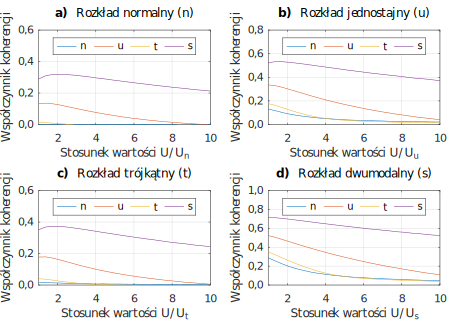
\includegraphics{obrazki/shapes}
\makecaption{fig:unc_shapefac}{Zależność wartości współczynnika koherencji w funkcji stosunku wartości niepewności rozszerzonej dla pary nieskorelowanych sygnałów błędów}
\end{center}
\end{figure}

Biorąc pod uwagę współczynnik kształtu dla pary rozkładów o identycznych wartościach niepewności rozszerzonej, opisany równaniem~\eqref{eq:unc_shapertwo}, korektę wynikającą z dysproporcji pomiędzy wartościami niepewności rozszerzonych sumowanych sygnałów opisaną równaniem~\eqref{eq:unc_cohercorra} oraz korektę wynikającą z założeń centralnego twierdzenia daną zależnością~\eqref{eq:unc_cohercorrb}, otrzymuje się zależność umożliwiającą oszacowanie wartości współczynników koherencji dla $N$ nieskorelowanych sygnałów błędów w postaci:
\begin{equation}
h_{i,j} = h_{j,i} = s_{i,j} \cdot p_{i,j} \cdot k_{i,j} = s_{i,j} \sqrt{\frac{\min \emb{U_{i}, U_{j}}}{\max \emb{U_{i}, U_{j}}}} \left( \frac{U_{i}^{2} + U_{j}^{2}}{\sum _{k = 0} ^{N-1} U_{k}^{2}} \right) \label{eq:unc_coher}.
\end{equation}
Na podstawie przedstawionego równania istnieje możliwość budowy macierzy koherencji, wykorzystywanej do wyznaczenia wypadkowej wartości niepewności rozszerzonej dla analizowanych sygnałów błędów zgodnie z zależnością~\eqref{eq:unc_matrix}. Należy zauważyć, że z uwagi na okoliczność możliwości wyznaczenia wartości współczynników kształtu $s_{i,j}$ niezależnie od parametrów niepewności błędów występujących w analizowanym torze pomiarowym, zaproponowana metoda jest możliwa do stosowania w czasie działania systemu również w przypadkach, gdy parametry te ulegają zmianie. Wadą przedstawionego rozwiązania jest konieczność wstępnego wyznaczenia wartości współczynników kształtu dla wszystkich rodzajów rozkładów sygnałów błędów występujących w analizowanym torze pomiarowym. Dodatkowo, ze względu na uproszczoną formę równania~\eqref{eq:unc_cohercorra}, która nie oddaje w pełni charakteru zależności przedstawionych na rysunku~\ref{fig:unc_shapefac}, wartości oszacowanych współczynników koherencji mogą być obarczone błędem, co w efekcie będzie miało wpływ na pojawienie się błędu oszacowania wartości wypadkowej niepewności rozszerzonej.

Ostatnim wymagającym komentarza przypadkiem jest przypadek, w którym istnieją korelacje pomiędzy analizowanymi sygnałami. Zgodnie z właściwościami macierzy koherencji elementy tej macierzy, podobnie jak elementy macierzy korelacji stosowanej w równaniu~\eqref{eq:var_matrix}, przyjmować mogą wartości z zakresu $<-1;1>$. Dla pełnej dodatniej korelacji wartość współczynnika koherencji wynosić będzie $1$, natomiast dla pełnej ujemnej korelacji wartość ta wyniesie $-1$~\cite{jakubiec_redmono}. W pozostałych przypadkach, zgodnie z informacjami przytoczonymi w poprzedniej części podrozdziału, wartość współczynnika koherencji wynikać będzie z wypadkowych parametrów kształtu splatanych rozkładów oraz współczynnika korelacji. Wobec powyższych nie jest możliwe oszacowanie wartości tego współczynnika stosując metody podobne do zaproponowanych w równaniach od~\eqref{eq:unc_shapertwo} do~\eqref{eq:unc_cohercorrb}. W omawianych sytuacjach, do wyznaczania wartości współczynników koherencji, zastosować należy metodę opisaną w pracy~\cite{jakubiec_reductive}. Inną alternatywą może być również przeprowadzenie analizy z osobna dla grup skorelowanych sygnałów, a następnie wykorzystanie wyznaczonych parametrów w równaniu~\eqref{eq:unc_matrix}.

Aby zweryfikować zasadność przedstawionych zależności przeprowadzono eksperyment metodą Monte-Carlo, którego celem było porównanie wartości niepewności rozszerzonej $U_{s}$ uzyskiwanej na drodze eksperymentu, zgodnie z instrukcją~\cite{jcgm_montecarlo}, oraz wartości $U_{c}$ uzyskiwanych zgodnie z równaniem~\eqref{eq:unc_matrix} dla współczynników koherencji wyznaczanych na podstawie równania~\eqref{eq:unc_coher}. Błąd względny $\delta_{U}$ oszacowania wartości niepewności rozszerzonej, wyrażony w procentach, będzie zatem definiowany w postaci:
\begin{equation}
\delta_{U} =  \frac{U_{c} - U_{s}}{U_{s}} \cdot 100\% \label{eq:unc_error}.
\end{equation}
W ramach eksperymentu generowano $N$ niezależnych sygnałów, których realizacje pobierane były z populacji o rozkładach $c_{i}$ i parametrach niepewności rozszerzonej $U_{i}$, których kolejne realizacje sumowano:
\begin{equation}
e_{\Sigma} \emb{k} = \sum _{i=0} ^{N-1} e_{i} \emb{k} \label{eq:unc_testsignal}.
\end{equation}
Dla uzyskanego sygnału, składającego się ze stu tysięcy próbek, wyznaczano niepewność rozszerzoną $U_{s}$ zgodnie z równaniem~\eqref{eq:unc_summation} oraz wartość $U_{c}$ oszacowaną na podstawie równania~\eqref{eq:unc_matrix} w celu wyznaczenia zgodnie z równaniem~\eqref{eq:unc_error} względnego błędu oszacowania wartości analizowanej wielkości. Opisywany proces powtarzano sto tysięcy razy, przy czym wartość $N$ pobierana była dla każdej iteracji z populacji danej przedziałem $<3,9>$ o jednakowym prawdopodobieństwie uzyskania każdej z wartości. Populacje kolejnych sygnałów $e_{i}$ stanowiły losowo kombinację rozkładów: normalnego, jednostajnego, trójkątnego i dwumodalnego, natomiast wartości niepewności rozszerzonej $U_{i}$ losowane były z przedziału $<U_{min};U_{max}>$ o jednakowym prawdopodobieństwie uzyskania każdej z wartości. Aby zweryfikować, w jakim stopniu zaproponowany w równaniu~\eqref{eq:unc_cohercorra} współczynnik korekty wpłynął na skuteczność opisanej w równaniu~\eqref{eq:unc_matrix} metody, eksperyment przeprowadzono dwukrotnie: stosując wartości współczynników koherencji wyznaczanych zgodnie z równaniem~\eqref{eq:unc_cohercorra} oraz po raz drugi, przyjmując wartość $p_{i,j} = 1$ dla dowolnej kombinacji $i$ oraz $j$. Na podstawie uzyskiwanych realizacji błędu opisanego równaniem~\eqref{eq:unc_error} sporządzano histogramm na którego podstawie oszacowano niepewność rozszerzoną analizowanej wielkości.

Ze względu na dużą zmienność parametrów sumowanych sygnałów zaproponowany eksperyment powinien w sposób miarodajny określić typową rozbieżność pomiędzy rzeczywistą, a oszacowaną za pomocą omawianej metody wartością niepewności rozszerzonej. Rysunek~\ref{fig:hist_reductive} przedstawia uzyskane histogramy względnego błędu oszacowania wypadkowej wartości niepewności rozszerzonej, natomiast w tabeli~\ref{tab:comp_reductive} przedstawiono porównanie uzyskanych wartości niepewności rozszerzonej błędu oszacowania wartości wypadkowej niepewności rozszerzonej w zależności od stosowania korekty zaproponowanej w równaniu~\eqref{eq:unc_cohercorra}, wyznaczone zgodnie z~\cite{jcgm_guide, jcgm_montecarlo}. Analizując wyniki przeprowadzonego eksperymentu zauważyć można, że wprowadzenie proponowanej korekty powoduje zmniejszenie szacowanej wartości niepewności rozszerzonej, a także zmniejszenie rozrzutu względnego błędu oszacowania tej wielkości. W efekcie możliwe jest oszacowanie wartości wypadkowej niepewności rozszerzonej z błędem względnym mieszczącym się w przedziale $<-5;5> \%$.

\begin{table}[htb!]
\begin{center}
\makecaption{tab:comp_reductive}{Zestawienie wartości niepewności względnego błędu szacowania wypadkowej wartości niepewności rozszerzonej w zależności od stosowania zaproponowanej w pracy korekty współczynnika kształtu}
\begin{tabular}[c]{| c | S[table-format = +1.2] | S[table-format = +1.2] | S[table-format = +1.2] | S[table-format = +1.2] | S[table-format = +1.2] | S[table-format = +1.2] | S[table-format = +1.2] | S[table-format = +1.2] |} \hline
\textbf{$U_{i}$} & \multicolumn{2}{c|}{\textbf{a) $<1;3>$}} & \multicolumn{2}{c|}{\textbf{b) $<1;6>$}} & \multicolumn{2}{c|}{\textbf{c) $<1;10>$}} & \multicolumn{2}{c|}{\textbf{d) $<1;20>$}} \\ \hline
\textbf{$\delta_{U}$} & \textbf{$U_{-}$} & \textbf{$U_{+}$} & \textbf{$U_{-}$} & \textbf{$U_{+}$} & \textbf{$U_{-}$} & \textbf{$U_{+}$} & \textbf{$U_{-}$} & \textbf{$U_{+}$} \\ \hline
Z korektą   & -2.23 & +4.83 & -2.43 & +4.59 & -2.54 & +4.52 & -2.62 & +4.45 \\ \hline
Bez korekty & -1.14 & +7.96 & -1.13 & +8.69 & -1.09 & +8.80 & -1.13 & +8.86 \\ \hline
\end{tabular}
\end{center}
\end{table}

\begin{figure}[htb!]
\begin{center}
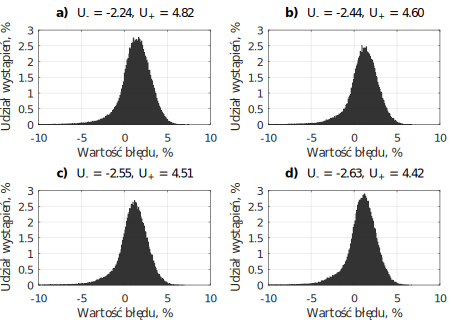
\includegraphics{obrazki/hist_reductive}
\makecaption{fig:hist_reductive}{Histogramy względnego błędu oszacowania wypadkowej wartości niepewności rozszerzonej dla zaproponowanej w pracy metody odpowiadające danym zestawionym w tabeli~\ref{tab:comp_reductive}}
\end{center}
\end{figure}

Analizując przedstawione dotychczas zależności zauważyć można, że sposób opisu niedokładności wyniku pomiaru zależeć będzie w dużej mierze od potrzeb projektanta toru pomiarowego oraz od specyfiki zakłócających proces pomiaru zjawisk. Opis wykorzystujący wariancję błędów wydaje się bardziej przystępny i mniej skomplikowany, a dodatkowo wariancja może być utożsamiana z mocą sygnału~\cite{proakis_dsp}. Opis wykorzystujący niepewność rozszerzoną będzie jednak bardziej precyzyjny, ze względu na informacje odnośnie prawdopodobieństwa wystąpienia danej wartości realizacji sygnału błędu, natomiast wymaga on większego zaangażowania w proces wyznaczania ostatecznej wartości tej wielkości. W odpowiednich okolicznościach, jeżeli spełnione są warunki związane z centralnym twierdzeniem granicznym, opis bazujący na wariancji sygnału błędu może być w łatwy sposób przeniesiony na opis związany z niepewnością rozszerzoną. Podczas wyznaczania wypadkowej wartości niepewności rozszerzonej stosować można metodę redukcyjnej arytmetyki interwałowej, opisaną szerzej w~\cite{jakubiec_reductive, jakubiec_redmono, batko_uncertainty}. Wyznaczone wartości niepewności rozszerzonej mogą w niewielkim stopniu odbiegać od wartości rzeczywistych, co opisano w~\cite{jakubiec_arithmetic, jakubiec_model}. Przyjmuje się jednak, że różnice nie przekraczające $5\%$ wartości prawdziwej są akceptowalne. Zaproponowana w równaniu~\eqref{eq:unc_cohercorra} zmniejsza omawiane różnice, zapewniając jednocześnie niski stopnień skomplikowania obliczeń. Można zatem stwierdzić, że zaproponowana w pracy metoda szacowania wypadkowej wartości niepewności rozszerzonej jest zasadna z punktu widzenia przyjętych założeń.

\section{Algorytm jako fragment toru pomiarowego}

Podczas opisu właściwości cyfrowej części toru pomiarowego przedstawiono przypadek, w którym analizowany obiekt przetwarzał kolejne próbki sygnału wejściowego na próbki sygnału wyjściowego zgodnie z odpowiadającą mu transmitancją i funkcją przetwarzania. Algorytmy stosowane w torach pomiarowych mogą generować wiele wielkości wyjściowych, pobierając przy tym w oknie pomiarowym określoną liczbę próbek wielkości wejściowych. W przypadku, gdy wyjście analizowanego obiektu stanowi $M$ próbek wielkości wyjściowych wyznaczanych na podstawie $N$ próbek wielkości wejściowych, a funkcja przetwarzania tego obiektu jest liniowa, działanie obiektu przedstawić można w ogólnej postaci jako~\cite{jakubiec_algorithms, jakubiec_single}:
\begin{equation}
\begin{bmatrix}
X \emb{0}   \\
X \emb{1}   \\
\vdots      \\
X \emb{M-1}
\end{bmatrix}
=
\begin{bmatrix}
a_{0, 0}   &   a_{0, 1} &   \cdots   &   a_{0, N-1}      \\
a_{1, 0}   &   \ddots   &            &   a_{1, N-1}      \\
\vdots     &            &   \ddots   &   \vdots          \\
a_{M-1, 0} &   \cdots   &   \cdots   &   a_{M-1, N-1}
\end{bmatrix}
\begin{bmatrix}
x \emb{0}   \\
x \emb{1}   \\
\vdots      \\
x \emb{N-1}
\end{bmatrix}
\label{eq:alg_out_mat},
\end{equation}
gdzie $a_{i,j}$ to kolejne współczynniki macierzy transformacji. Równanie~\eqref{eq:alg_out_mat} można przedstawić również w postaci iloczynu:
\begin{equation}
\mathbf{X} = \mathbf{A} \cdot \mathbf{x} \label{eq:alg_out_mul},
\end{equation}
gdzie $\mathbf{X}$ jest wektorem wielkości wyjściowych, $\mathbf{A}$ macierzą transformacji oraz $\mathbf{x}$ wektorem wielkości wejściowych~\cite{jakubiec_algorithms}. Wobec przedstawionych zależności, pojedynczą wielkość wyjściową algorytmu przedstawić można w postaci:
\begin{equation}
X \emb{i} = a_{i, 0} x \emb{0} + a_{i, 1} x \emb{1} + \hdots + a_{i, N-1} x \emb{N-1} \label{eq:alg_out_single}.
\end{equation}
Na podstawie przedstawionych zależności zauważyć można, że analizowany obiekt stanowi w zasadzie zbiór filtrów o skończonej odpowiedzi impulsowej \enquote{FIR}. Przedstawione metody analizy będą zatem przypominały metody analizy opisywanego typu filtru~\cite{mehrnia_fir}.

W praktyce wartości współczynników macierzy transformacji opisanej równaniem~\eqref{eq:alg_out_mat} mogą nie być znane przez projektanta toru pomiarowego. Ich znajomość jest jednak konieczna w celu przeprowadzenia analizy metrologicznej zastosowanego algorytmu. Najczęściej projektant toru pomiarowego stosuje gotowy algorytm, zaimplementowany np. w środowisku \enquote{GNU Octave} lub dostarczany mu jako zewnętrzną bibliotekę. W takim przypadku należy przeprowadzić proces identyfikacji wartości współczynników macierzy, który przedstawiony zostanie w dalszej części rozdziału. Innym przypadkiem jest sytuacja, w której z punktu widzenia analizy metrologicznej macierzowy opis algorytmu jest korzystny, a wartości współczynników mogą być wyznaczone za pomocą odpowiednich funkcjonałów. Ostatnim przypadkiem jest sytuacja, w której znana jest transmitancja $H(z)$ dla kolejnych wielkości wyjściowych. Wtedy wyznaczenie wartości współczynników macierzy transformacji odbywać się będzie poprzez przekształcenie tej transmitancji na postać zgodną z równaniem~\eqref{eq:alg_out_single}. Należy jednak zauważyć, że nie we wszystkich przypadkach przedstawione metody znajdują zastosowanie.

W przypadku, gdy dysponuje się gotową implementacją algorytmu, w celu identyfikacji współczynników macierzy transformacji należy podawać na wejście algorytmu wektor wielkości wejściowych, którego wszystkie elementy poza wybranym mają wartość zero. Wartość jednego elementu należy ustawić na jeden, a następnie za pomocą identyfikowanego algorytmu wyznaczyć należy wektor wielkości wyjściowych. Wyznaczony wektor stanowi kolumnę identyfikowanej macierzy transformacji, przy czym numer kolumny jest równy indeksowi elementu, który w wektorze wielkości wejściowych posiadał wartość jeden. W celu wyznaczenia wszystkich wartości macierzy transformacji należy powtórzyć powyższą czynność dla wektorów wartości wejściowych algorytmu zgodnie z zależnością~\cite{jakubiec_algorithms}:
\begin{equation}
x \emb{n} =
\begin{cases}
	1 & $gdy$~n = i \\
	0 & $gdy$~n \neq i
\end{cases}
\label{eq:wt_ident},
\end{equation}
dla $i$ w przedziale $<0;N-1>$, gdzie $i$ jest indeksem identyfikowanej kolumny macierzy transformacji. Niezależnie od struktury numerycznej analizowanego obiektu opisana metoda jest uniwersalna, przy czym wymaga ona, aby identyfikowany algorytm spełniał założenia przedstawione na początku podrozdziału.

Aby ustalić związek pomiędzy błędami wielkości wejściowych, a błędami wielkości wyjściowych analizowanego algorytmu należy przeanalizować proces wyznaczania wartości pojedynczej wielkości wyjściowej tego algorytmu. Wobec tego, jeżeli wielkości wejściowe algorytmu są obarczone błędami o charakterze addytywnym zgodnie z zależnością:
\begin{equation}
\tilde{x} \emb{i} = \dot{x} \emb{i} + e_{x,\Sigma} \emb{i} = \dot{x} \emb{i} + e_{x,s} \emb{i} + e_{x,d} \emb{i} + e_{x,r} \emb{i} \label{eq:alg_inputval},
\end{equation}
gdzie $e_{x,s}$ oznacza błąd statyczny, $e_{x,d}$ błąd dynamiczny oraz $e_{x,r}$ błąd losowy wielkości wejściowej, to istnieje możliwość osobnej analizy wyniku algorytmu dla idealnych wartości wielkości wejściowych oraz dla związanych z nimi błędów. Błąd wielkości wyjściowej przenoszony z wejścia na wyjście algorytmu można zatem opisać, zgodnie z równaniem~\eqref{eq:alg_out_single}, jako kombinację liniową współczynników transformacji algorytmu oraz błędów wielkości wejściowych:
\begin{equation}
e_{X,p} \emb{i} = a_{i, 0} e_{x,\Sigma} \emb{0} + a_{i, 1} e_{x,\Sigma} \emb{1} + \hdots + a_{i, N-1} e_{x,\Sigma} \emb{N-1} \label{eq:alg_outerr}.
\end{equation}

Dla błędów o charakterze statycznym, ze względu na fakt że realizacja tych błędów jest niezmienna w obrębie okna pomiarowego, równanie~\eqref{eq:alg_outerr} można uprościć i zapisać w postaci:
\begin{equation}
e_{X,s} \emb{i} = a_{i, 0} e_{x,s} + a_{i, 1} e_{x,s} + \hdots + a_{i, N-1} e_{x,s} = e_{x,s} \sum _{j = 0} ^{N-1} a_{i, j} \label{eq:alg_outerr_stat},
\end{equation}
gdzie $e_{x,s}$ jest błędem statycznym wielkości wejściowej, natomiast $e_{X,s}$ błędem statycznym wielkości wyjściowej algorytmu. Powtarzając pomiar wielokrotnie, dla różnych pozycji okna pomiarowego, realizacje błędu statycznego mogą przyjmować różne wartości. W takim przypadku wyjściowy błąd statyczny również można rozpatrywać w kategoriach probabilistycznych, a jego wariancję opisać można równaniem uwzględniającym wariancję wejściowego błędu statycznego:
\begin{equation}
\sigma_{X,s}^{2} \emb{i} = \sigma_{x,s}^{2} \left( a_{i, 0} + a_{i, 1} + \hdots + a_{i, N-1} \right)^{2} = \sigma_{x,s}^{2} \left( \sum _{j = 0} ^{N-1} a_{i, j} \right)^{2} \label{eq:alg_outvar_stat}.
\end{equation}
Należy zauważyć, że kształt rozkładu wyjściowego błędu statycznego będzie identyczny, jak kształt rozkładu statycznego błędu wejściowego.

Dla błędów o charakterze dynamicznym należy przeprowadzić analizę zgodnie z metodologią przedstawioną w poprzedniej części rozdziału, wykorzystując znajomość transmitancji $H(z)$ odpowiedniej dla analizowanej wielkości wyjściowej algorytmu. Identycznie, jak w przypadku równania~\eqref{eq:mid_disc_err_dyn_prop}, wyznaczyć należy wypadkowe amplitudy oraz przesunięcia w fazie kolejnych harmonicznych błędu dynamicznego, a następnie złożyć je zgodnie z zależnością~\eqref{eq:dyn_multi}. Transmitancja $H(z)$ dla $i$-tej wielkości wyjściowej może zostać wyznaczona na podstawie wartości współczynników $i$-tego wiersza macierzy transformacji algorytmu jako:
\begin{equation}
H_{i} \emb{z} = a_{i, 0} + a_{i, 1} z^{-1} + \hdots + a_{i, N-1} z^{-N+1} = \sum _{k = 0} ^{N-1} a_{i, k} z^{-k} \label{eq:alg_trans_single}.
\end{equation}
W omawianym przypadku przyjmuje się, że algorytm posiada idealną transmitancję, a ewentualne rozbieżności nie mają wpływu na widmo przenoszonego sygnału. Dodatkowe informacje związane z tym zagadnieniem zostaną przedstawione w dalszej części podrozdziału.

W przypadku błędów o charakterze losowym, wykonując algorytm wielokrotnie, uzyskać można zależność wiążącą wariancję błędu na wyjściu algorytmu z wariancją błędów wielkości wejściowych. Zakładając, że wszystkie wielkości wejściowe algorytmu pochodzą z tej samej cześć toru pomiarowego, a zatem ich parametry statystyczne są identyczne, oraz że kolejne błędy wielkości wejściowych nie są ze sobą skorelowane, zależność tą opisać można jako:
\begin{equation}
\sigma_{r}^{2} \emb{i} = a_{i, 0}^{2} \sigma_{x,r}^{2} + a_{i, 1}^{2} \sigma_{x,r}^{2} + \hdots + a_{i, N-1}^{2} \sigma_{x,r}^{2} = \sigma_{x,r}^{2} \sum _{j=0} ^{N-1} {a_{i, j}^{2}} \label{eq:alg_outvar_rand}.
\end{equation}

Poza przenoszeniem przez algorytm błędów zawartych w wielkościach wejściowych na jego wyjście, algorytm wprowadza do wielkości wyjściowych błędy własne. Błędy te wynikają niedokładności wyznaczenia współczynników algorytmu oraz z przeprowadzanych podczas obliczeń zaokrągleń. Ich wartości będą zatem uzależnione od wielu czynników, a ich analiza powinna odbywać się indywidualnie dla zaimplementowanego algorytmu. Zakładając, że wyznaczanie wartości $i$-tej wielkości wyjściowej algorytmu odbywać się będzie wielokrotnie, błędy własne opisywać można w kategorii probabilistycznej za pomocą związanej z nimi wariancji $\sigma_{X,z}^{2}(i)$. Ze względu na fakt, że liczba operacji mnożenia i dodawania, odpowiedzialnych za powstawanie omawianej grupy błędów będzie duża ($N$ mnożeń oraz $N$ dodawań) błąd ten będzie miał rozkład zbliżony do normalnego~\cite{jcgm_guide}. W przypadku, gdy na etapie identyfikacji wartości macierzy współczynników uzyskano wartości obarczone błędami, należy rozszerzyć analizę o przedstawienie konsekwencji tego zjawiska. W takim przypadku należy przeanalizować wprowadzany do wielkości wyjściowych statyczny błąd własny oraz wykonać analizę dla błędów własnych dynamicznych, analogicznie jak opisano równaniem~\eqref{eq:mid_disc_err_dyn_self}. Omawiany przypadek nie będzie rozpatrywany w pracy, ponieważ identyfikując wartości macierzy transformacji za pomocą przedstawionego algorytmu lub wyznaczając ich wartości przy użyciu odpowiednich funkcjonałów, wprowadzany błąd wynikać będzie głównie z zaokrągleń i będzie można analizować go równolegle z wprowadzanym losowym błędem $e_{X,z}$. Omawianą analizę przedstawia szczegółowo praca~\cite{jakubiec_system}.

Wobec powyższych założeń, w celu wyznaczenia wariancji $\sigma_{X,\Sigma}^{2}(i)$ wypadkowego błędu $e_{X,\Sigma}(i)$ dla $i$-tej wielkości wyjściowej analizowanego algorytmu należy wykorzystać zależność~\eqref{eq:var_matrix}, przy czym przyjmuje ona w tym przypadku postać:
\begin{equation}
\sigma_{X,\Sigma}^{2} \emb{i} =
\begin{bmatrix}
\sigma_{X,s} \emb{i} \\ \sigma_{X,d} \emb{i} \\ \sigma_{X,r} \emb{i} \\ \sigma_{X,z} \emb{i}
\end{bmatrix}^{T}
\begin{bmatrix}
1         & r_{d,s} & r_{r,s} & r_{z,s} \\
r_{s,d}   & 1       & r_{r,d} & r_{z,d} \\
r_{s,r}   & r_{d,r} & 1       & r_{z,r} \\
r_{s,z}   & r_{d,z} & r_{r,z} & 1
\end{bmatrix}
\begin{bmatrix}
\sigma_{X,s} \emb{i} \\ \sigma_{X,d} \emb{i} \\ \sigma_{X,r} \emb{i} \\ \sigma_{X,z} \emb{i}
\end{bmatrix}
\label{eq:alg_outvar_mat},
\end{equation}
gdzie $r_{i,j}$ stanowi współczynnik macierzy korelacji dla wybranych błędów cząstkowych analizowanego algorytmu. Wyznaczenie niepewności rozszerzonej może być przeprowadzone zgodnie z zależnością~\eqref{eq:unc_matrix}, przekształconą do postaci:
\begin{equation}
U_{X,\Sigma} \emb{i} = \sqrt{
\begin{bmatrix}
U_{X,s} \emb{i} \\ U_{X,d} \emb{i} \\ U_{X,r} \emb{i} \\ U_{X,z} \emb{i}
\end{bmatrix}^{T}
\begin{bmatrix}
1         & h_{d,s} & h_{r,s} & h_{z,s} \\
h_{s,d}   & 1       & h_{r,d} & h_{z,d} \\
h_{s,r}   & h_{d,r} & 1       & h_{z,r} \\
h_{s,z}   & h_{d,z} & h_{r,z} & 1
\end{bmatrix}
\begin{bmatrix}
U_{X,s} \emb{i} \\ U_{X,d} \emb{i} \\ U_{X,r} \emb{i} \\ U_{X,z} \emb{i}
\end{bmatrix}}
\label{eq:alg_outunc_mat},
\end{equation}
przy czym $h_{i,j}$ oznacza współczynnik koherencji wyznaczany zgodnie z zależnością~\eqref{eq:unc_coher}. Należy zauważyć, że równania~\eqref{eq:alg_outvar_mat} oraz~\eqref{eq:alg_outunc_mat} mogą zawierać inną liczbę elementów, niż wskazano. Dokładna postać przedstawionych równań zależeć będzie od budżetu niepewności wielkości wejściowych analizowanego algorytmu.

Na podstawie równań~\eqref{eq:alg_outvar_stat} oraz~\eqref{eq:alg_outvar_rand} wprowadzić można dodatkowe wielkości przedstawione następującymi zależnościami:
\begin{gather}
A_{i,s} = \sum _{j = 0} ^{N-1} a_{i, j} \label{eq:alg_trans_stat}, \\
A_{i,r} = \sqrt{\sum _{j = 0} ^{N-1} a_{i, j}^{2}} \label{eq:alg_trans_rand},
\end{gather}
gdzie $A_{i,s}$ jest współczynnikiem przenoszenia dla błędów statycznych, natomiast jest $A_{i,r}$ współczynnikiem przenoszenia dla błędów losowych $i$-tej wielkości wyjściowej analizowanego algorytmu. Wyznaczenie wartości opisanych współczynników umożliwi wyznaczenie wariancji kolejnych błędów losowych oraz statycznych, a dodatkowo będzie stanowiło informacje, w jaki sposób analizowany algorytm przenosi z wejścia na wyjście określony rodzaj błędu. Można zauważyć, że dla niskich wartości współczynnika przenoszenia (tj. $A_{i} < 1$) kolejne błędy wielkości wejściowych będą tłumione (wariancja błędu wielkości wyjściowej będzie mniejsza, niż wariancja błędów wielkości wejściowych). Odwrotna sytuacja będzie miała miejsce w przypadku dużych wartości współczynnika (tj. $A_{i} > 1$).

W przypadku analizy błędów dynamicznych, na podstawie równania~\eqref{eq:alg_trans_single} po podstawieniu $z = e^{j\omega}$, wyznaczyć można adekwatne dla równań~\eqref{eq:mid_disc_amp} oraz~\eqref{eq:mid_disc_phi} zależności opisujące wzmocnienie $K_{X,i}(\omega_{n})$ oraz przesunięcie w fazie $\varphi_{X,i}(\omega_{n})$ przetwarzanych harmonicznych sygnału w funkcji pulsacji znormalizowanej $\omega_{n}$ dla $i$-tej wielkości wyjściowej algorytmu w postaci:
\begin{gather}
G_{X,i} \emb{\omega_{n}} = \sum _{k = 0} ^{N-1} a_{i,k} e^{-j k \omega_{n}} \label{eq:alg_trans_norm}, \\
K_{X,i} \emb{\omega_{n}} = \left| G_{X,i} \emb{\omega_{n}} \right| = \sqrt{\left( \Re \left( G_{X,i} \emb{\omega_{n}} \right) \right)^{2} + \left( \Im \left( G_{X,i} \emb{\omega_{n}} \right) \right)^{2}} \label{eq:alg_trans_amp}, \\
\varphi_{X,i} \emb{\omega_{n}} = \arctan \left( \frac{\Im \left( G_{X,i} \emb{\omega_{n}} \right)}{\Re \left( G_{X,i} \emb{\omega_{n}} \right)} \right) \label{eq:alg_trans_phi},
\end{gather}
przy czym pulsacja znormalizowana, oznaczona symbolem $\omega_{n}$, odnosi się do pulsacji próbkowania i jest określona przez następującą zależność:
\begin{equation}
\omega_{n} = 2\pi \frac{\omega}{\omega_{s}} \label{eq:puls_norm},
\end{equation}
gdzie $\omega$ jest analizowaną pulsacją, natomiast $\omega_{s}$ pulsacją próbkowania równą $\frac{2 \pi}{T_{p}}$ dla okresu próbkowania $T_{p}$. Prawidłowa wartość pulsacji znormalizowanej mieści się zatem w zakresie $<0;\pi>$, co odpowiada zakresowi od zera do pulsacji Nyquista dla przyjętego okresu próbkowania.

\section{Podsumowanie przedstawionych zależności}

W poprzednich częściach rozdziału przedstawiono modele kolejnych fragmentów toru pomiarowego, które opisywały związki pomiędzy błędami na wejściu i wyjściu analizowanego obiektu, a także wskazywały rolę tego obiektu we wprowadzaniu do sygnału wyjściowego błędów własnych. Zaproponowany model wprowadzał podział na statyczne i dynamiczne właściwości obiektu, które opisywane były transmitancją i funkcją przetwarzania obiektu. Opisane zaproponowanym modelem fragmenty toru pomiarowego, które zostały ze sobą połączone kaskadowo oraz cechują się addytywną funkcją przetwarzania, opisać można modelem wypadkowym oraz z osobna analizować zawarte w nim błędy cząstkowe. Zaproponowana metoda wyznaczania niepewności wypadkowej bazuje na określeniu związków pomiędzy kolejnymi niepewnościami składowymi, a następnie wykorzystuje redukcyjną arytmetykę interwałową do wyznaczenia niepewności wypadkowej. Zaproponowany opis uwzględnia ewentualne korelacje pomiędzy kolejnymi grupami błędów, a w przypadku braku tych korelacji wymaga jedynie określenia związków pomiędzy kształtem rozkładu kolejnych składanych błędów~\cite{jakubiec_reductive, batko_uncertainty}.

Przedstawiony model oceny dokładności wyniku pomiaru zakłada, że obecne w sygnale pomiarowym błędy cechują się symetrycznymi rozkładami o zerowej wartości oczekiwanej. W przypadku, gdy wartość oczekiwana realizacji błędu jest niezerowa, błąd ten posiada składową systematyczną, którą należy skorygować w ostatecznym wyniku pomiaru. Jeżeli nie jest spełnione założenie odnośnie symetrii rozkładów składanych błędów, to do określenia rozkładu błędu wynikowego należy stosować metodę analityczną bazującą na wyznaczeniu splotu składanych funkcji gęstości prawdopodobieństwa lub wykorzystać metodę Monte-Carlo, która jest zwykle bardziej przystępna i optymalna ze względu na mniejszy stopień skomplikowania~\cite{janssen_montecarlo, roj_annuncertainty}.

Przeprowadzone rozważania nie poruszały problemu opóźnień w systemach pomiarowo-sterujących, a zatem nie brano w nich pod uwagę błędów związanych z opóźnieniami. Tematyka ta nie będzie poruszana w dalszych częściach pracy. Warto jednak zauważyć, że zaproponowany model błędu może być z łatwością dopasowany do możliwości analizy właściwości i wpływu tych błędów na niedokładność wielkości wyjściowych. Należy wtedy uwzględnić w modelu dodatkowy składnik błędu, który definiować można zgodnie z metodą zaproponowaną w~\cite{wymyslo_delay, jakubiec_system}. Z punktu widzenia zaproponowanego modelu, zjawisko to opisać można jako dodatkowe przesunięcie w fazie składowych przetwarzanego sygnału, będące iloczynem pulsacji analizowanej harmonicznej i wartości realizacji błędu opóźnienia.
